\documentclass{article}

%\usepackage{arxiv}
\usepackage[utf8]{inputenc} % allow utf-8 input
\usepackage[T1]{fontenc}    % use 8-bit T1 fonts
\usepackage{hyperref}       % hyperlinks
\usepackage{url}            % simple URL typesetting
\usepackage{booktabs}       % professional-quality tables
\usepackage{amsfonts}       % blackboard math symbols
\usepackage{amsmath} 
\usepackage{mlmodern}
\usepackage{nicefrac}       % compact symbols for 1/2, etc.
\usepackage{microtype}      % microtypography
\usepackage{lipsum}
\usepackage{natbib}
\bibpunct[: ]{(}{)}{;}{a}{,}{;}
\usepackage{setspace}
\usepackage{graphicx}
\usepackage{placeins}
\usepackage{tabularx}
\usepackage[paper=portrait,pagesize]{typearea}


\usepackage[left=1in,right=1in,top=1in,bottom=1in]{geometry}

\usepackage{caption}
\usepackage{subcaption}


\title{A Field Experiment on Business Opposition to the U.S.-China Trade War\thanks{We thank each of the Princeton Niehaus Fellows of 2018 -  2019 who provided generous and valuable feedback on the research design: Shannon Carcelli, Marco Martini, Haillie Lee, Andrey Tomashevskiy, Quynh Nguyen, and In Song Kim. We also thank Marco Martini, Clayton Webb, and Jieun Lee for excellent comments, as well as audiences at the KU Trade War Lab Speaker Series, APSA 2021, IPES 2021, and at Wesleyan University. We thank the Niehaus Center for Globalization and Governance and the Charles Koch Foundation for generous financial support. We are also grateful to the Kansas City Chamber of Commerce and World Trade Center KC for helping us survey their members. For excellent research assistance, we thank Edmond Cheung, Quinn Lee, Peter Campbell, Shahab Mirza, Rebecca Russavage, Joshua Bennion, Mary Harris, Jena Burgess, Sean O'Hara, and Lisie O'Hara. All errors are our own.}}

\author{
 Lindsay R. Dolan\thanks{
 Department of Government,
  Wesleyan University, Email:
  \texttt{ldolan@wesleyan.edu}. Authors are currently listed in alphabetical order.}
  \and
  Robert M. Kubinec \thanks{
  Division of Social Sciences,
  New York University Abu Dhabi, Email:
  \texttt{rmk7@nyu.edu}}
  \and
  Daniel L. Nielson \thanks{
  Department of Government,
  University of Texas at Austin, Email:
  \texttt{dan.nielson@utexas.edu}}
  \and
  Jiakun J. Zhang \thanks{
  Department of Political Science,
  University of Kansas, Email:
  \texttt{jiakunzhang@ku.edu}
  }
}

\date{\today}

\pagenumbering{gobble}

\begin{document}

\maketitle


\begin{abstract}
\noindent

%edited version:

\noindent Despite the harmful consequences of the U.S-China trade war, only a handful of firms took collective action to oppose it. To understand why, we implemented a field experiment in which we randomly provided detailed estimates of the costs of the trade war to U.S. company managers and measured their willingness to take actions either opposing or supporting the trade war. While overall our treatment counter-intuitively reduced opposition to the trade war, these effects were highly conditional on respondents' prior beliefs and the number of tariffs in their industry. The treatment increased opposition the most among subjects in industries with substantial tariffs who also thought the trade war was harmful. However, it decreased opposition among subjects who held neutral beliefs about the trade war. Finally, we find that a company’s political culture strongly predicts their political activity, suggesting political ideology and not just a company’s business interests shape corporate behavior.

%The trade war with China negatively impacted most U.S. companies, but only a handful of firms acted to oppose it. To understand corporate collective action, we implemented a field experiment in which we randomly provided original estimates of the costs of the trade war to managers of U.S. firms and then measured their willingness to take actions either opposing or supporting the trade war. While on the whole, our treatment reduced opposition to the trade war, these effects were highly conditional on respondents' prior beliefs and the number of tariffs in their industry. The treatment increased opposition the most among subjects in industries with substantial tariffs who also perceived the trade war as harmful. However, it decreased opposition among subjects who held neutral beliefs about the trade war. Finally, we find that a company’s political culture strongly predicts their political activity, suggesting ideological views and not just a company’s business interests shape corporate behavior.
%The United States's trade war with China proved to be detrimental to a wide swath of U.S. companies, but only a handful of well-connected firms pursued vigorous political action to oppose it. To better understand the constraints to corporate political action, we implemented a field experiment targeted at managers of U.S.-based firms in which we randomly provided original estimates of the costs of the trade war to their industry and company and then measured their willingness to take actions either opposing or supporting the trade war. We find that on the whole, U.S. companies that receive information about the rise in input costs from tariffs are less likely to take political action opposing the trade war, though this effect is highly conditional on respondents' pre-existing beliefs and on the number of tariffs affecting their industries. The information treatment caused the greatest opposition to the trade war among subjects who believed the trade war was harmful and whose companies' industries were affected by the largest array of tariffs. On the other side, subjects who previously believed they were helped by the trade war, and thus for whom the treatment provided contrasting evidence of trade-war harm from many tariffs, grew significantly less likely to support the trade war. Subjects with intermediate beliefs about the benefits or costs of the trade war showed the strongest negative effects from treatment. Finally, we find that the company's political culture was as strong a predictor of support for or against the trade war as was the company's own vulnerability to tariff-related cost increases, suggesting that ideological views strongly shaped pre-existing beliefs. (256 words)
\end{abstract}

\textbf{Keywords}: trade war, firms, field experiment

\bigskip
\begin{center}
    Word Count: 11,895
\end{center}


\doublespacing

\newpage

 \setcounter{page}{1}
 \pagenumbering{arabic}

\section{Introduction}

The trade wars waged by the Trump Administration since 2018, and now continued by the Biden Administration, resulted in unprecedented increases in tariffs affecting dozens of countries and thousands of products. It has upended the steel, aluminum, solar panel, washing machine, and auto industries, among many others. It has also affected nearly every business tie with China, with which the average tariff level has risen from 3 to 20 percent between 2017 and 2020. Economists estimate that these trade policies have primarily burdened U.S. consumers and businesses on the scale of \$4.6 billion per month, with \$165 billion worth of trade redirected to avoid tariffs \citep{amiti2019impact}. Indeed, survey data indicate broad opposition to the trade war among U.S. consumers and businesses.\footnote{Ben Casselman and Ana Swanson, ``Survey shows broad opposition to Trump trade policies,'' \textit{New York Times}, September 19, 2019. \url{https://www.nytimes.com/2019/09/19/business/economy/trade-war-economic-concerns.html}}

Political economists expect those most harmed by protectionism would act collectively to politically oppose the trade war \citep{milner1999political}. But we have seen relatively little broad-based political mobilization. \citet{zhu2021firms} estimate that just 1.73\% of all large firms in the U.S. have publicly opposed the tariffs. The absence of political mobilization is understandable for consumers, who---while being the main losers from tariffs---face diffuse costs that make it challenging for them to overcome collective-action problems. The real puzzle is why businesses, who are typically thought to be more active and able in trade policy, have not done more to demand an end to the tariffs.

To be sure, firms have not been silent. In early March 2018, the Business Roundtable made an unequivocal statement that the tariffs were an ``unforced error'' and would not succeed in protecting American jobs and workers.\footnote{https://www.businessroundtable.org/business-roundtable-statement-on-president-trumps-steel-and-aluminum-tariffs} By September 2018, 80 trade associations had joined together under the umbrella organization Americans for Free Trade, which has drafted numerous letters to the government. Historically, however, corporate political activity on trade policy has been more successful when petitions are filed by firms with heavy campaign contributions than through trade associations \citep{rehbein1994determining}. But individual firms affected by the trade war mostly dedicated their resources to seeking individualized exemptions from the tariffs, rather than pursuing policy change.\footnote{James Politi, ``US tariffs see small businesses plead for mercy as trade war bites,'' \textit{Financial Times}, August 23, 2018.}

What causes firms to engage in collective action to end (or prolong) a trade war? Answering this question is essential to understanding the political power that can be wielded by wealthy market actors. While a large literature investigates the strategic (Olson 1965), social \citep{gerber2008social}, and ideological reasons why individuals may take collective action, we know less about whether firms behave similarly.

For one, we question whether firms had good information about how the trade war would impact their operations. To be sure, many of the firms with certainty about the higher prices they faced filed thousands of requests to the United States Trade Representative (USTR) to be exempt from tariffs on highly specialized products that were not produced in the U.S. For example, according to an engineer at a fishing hook manufacturer, ``If we can't get the exemption, we will stop making that product altogether.'' Likewise, one employee of a manufacturer making precision gears for aerospace companies claimed that the specific grade of metal it imports from Europe is the only one strong enough to ensure safely constructed airplanes.\footnote{\url{https://www.marketplace.org/2018/04/25/economy/whos-asking-exemptions-trumps-tariffs}} For many firms, the costs were clear.

But others may not have been fully aware of the toll the trade war has taken on their business. Even economists have struggled to estimate the costs of the trade war. One reason for this is the complex global supply chains that amplify and yet conceal the effects of tariffs, presenting an empirical challenge to scholars who have sought to quantify the trade dispute's impact \citep{flaaen2019disentangling}. Another complication is that both U.S. protectionism and foreign retaliation appear to target certain politically valuable sectors and counties, and their net effect is often interactive and distorted \citep{fajgelbaum2020return}.

If economists have struggled to adequately model the consequences of the trade war, we expect firms to suffer from an even inferior informational environment. Consider this 2018 advice from the Boston Consulting Group:

\begin{quote}
Trade policy impact assessments are designed to look at the net welfare or GDP effects of higher tariffs. That is relevant for firms but often not the most important consideration. Firms want to understand the impact on their specific business and bottom line. This impact can be much higher than the overall welfare effect, and it can even go in the opposite direction. ...
Importantly, firms will differ in the way they are affected by trade policy action. Their exposure depends on the dynamics of the market segments on which they focus, the flexibility of their production systems, and the global footprint of their value chains. ... Firms need to boost their analytical capacity to prepare themselves to assess a more uncertain environment ahead and to prepare their responses in a fact-driven way.\footnote{Christian Ketels and Martin Reeves, ``How Much Will a Trade War Hurt Your Business?'' Boston Consulting Group, August 18, 2018. \url{https://www.bcg.com/publications/2018/how-much-will-trade-war-hurt-your-company.aspx}}
\end{quote}

We suspect that many firms lack this analytical capacity, and dedicating resources to developing it is yet another cost of the trade war. We implement what is, to the best of our knowledge, the first field experiment to manipulate firms' information base about the costs and benefits of policy and measure the treatment's consequences on real-world political behavior opposing or supporting tariffs. We tested whether providing the needed analytical capacity and informing managers about the impact of the trade war on their businesses increases the likelihood that they will undertake political action contacting leaders, joining collective initiatives, signing petitions, and donating to like-minded politicians. Our focus is on small and medium-sized enterprises (SMEs) and the modest but meaningful political actions they can take. SMEs have been profoundly impacted by the trade war, are less well-informed, employ a significant share of the American work force who engage in political behaviors, and are largely overlooked in studies of trade policy. 

We created a novel sample of managers at U.S. firms using social media targeting and outreach to U.S. Chambers of Commerce. Using supply tables from the Bureau of Economic Analysis, we calculate for each industry---based on the upstream industries on which it relies---the cost of the trade war, and we develop an interactive web application that allows firms to estimate this for themselves more precisely based on their own inputs and quantities. We collect information about the subject company managers' knowledge of the trade war and their beliefs about the harm or help that their companies received from the trade war. As an outcome measure, we ask whether the firms would want to undertake a number of behaviors to express either their opposition to or support for the current trade war.

We find, contrary to much thinking about the determinants of corporate political action, that presenting information about tariff-related input costs in the aggregate tends to depress rather than increase political action opposing the trade war. However, we find that this effect is highly conditional on the costs from tariffs and on prior beliefs of subjects on whether the trade war helped or harmed their firms. The treatment depressed political action the most among those with middling levels of knowledge and prior exposure to the trade war, a result we find puzzling and for which we can only offer speculation about its interpretation. In the clearest results, we find that subjects who previously believed the trade war harmed them and for whom the treatment augmented perceived costs from high numbers of tariffs, became significantly more likely to oppose the trade war, by as much as 40\%. On the other side, subjects who before treatment believed the trade war helped them but for whom the treatment provided strongly contrasting information indicating extensive economic harm from tariffs became significantly less likely to support the trade war.

In addition, we note that a firm's political culture was associated with very strong tendencies toward support or opposition to the trade war, with managers at liberal firms opposing the tariffs and managers at conservative firms supporting them. The observational correlations from these ideological leanings are very strong and suggest findings contrary to theories of political economy focusing on firm interests and comparative advantage. In what follows, we develop the theoretical motivation and expectations, describe the research design, present and discuss the results, and consider implications for policy and future scholarship.

% intro is already pretty long


%Our study complements a growing literature in economics on the 2018-present trade war \citep{amiti2019impact,amiti2020s,flaaen2019disentangling,fajgelbaum2020return,handley2020rising}
%by focusing on the political activities of firms. In doing so, we deepen scholarly understanding of collective action by applying experimental methods with a novel and important political player --- firms.

\section{Firms, Trade, and Political Behavior}

Trade produces winners and losers, and a large literature theorizes and investigates producers' preferences over trade policy. Factor endowment models of trade such as Heckscher-Ohlin suggest that preferences over trade will divide along factoral lines, with owners of the relatively abundant factor of production benefiting from and supporting free trade, while the relatively scarce factor opposes it \citep{rogowski1987political}. Sectoral models, including Ricardo-Viner, instead identify industries as the main cleavages that divide producers \citep{hiscox2002international}. Any individual associated with an industry that utilizes that relatively abundant factor of production should benefit from and support trade, irrespective of their personal factor endowment (labor or capital), while industries that utilize scarce factors of production should seek protection. But scholars increasingly suggest that producer preferences result from a given firm's exposure to global value chains. Firms that outsource their production processes would be heavily penalized by import limitations and should push for free trade to maximize the efficiency of their operations \citep{farrell2016new}. Indeed, \citet{kim2019firms2} survey firms in Costa Rica and find that GVC-connected firms placed greater value on trade liberalization.

It is therefore unsurprising that firms have had generally negative reactions to the trade war. \citet{lee2021firms} investigate the comments submitted to the U.S. Trade Representative. They find the comments to be overwhelmingly negative, and more likely to be submitted by firms with subsidiaries in China. This is consistent with the idea that firms act on their material interests, and specifically, their interests are more sensitive to their production networks than trade competition. Widespread tariffs have heavily penalized U.S. businesses that faced sometimes impracticable costs of sourcing materials, let alone exporting their products abroad, on top of a heavily bureaucratized and slow-moving tariff exemption process. Only a very few firms "won" --- steel giant AK Steel, for example --- and they were among the few firms that took action to prolong and expand the trade war. But although national political action by firms has overwhelmingly opposed rather than supported the trade war, 98.27\% of firms have not taken a public stand on the trade war \citep{zhu2021firms}.

We argue that many firms are unwilling to act on their preferences due to the costliness of collective action. Take a group of firms adversely affected by trade liberalization or protection. Most theories of collective action propose that the firms will undertake action only when the benefits they receive outweigh the costs of participation. When benefits are concentrated among a small group, the shared benefits that accrue to a single firm may be significant enough to compensate them for the costs of engagement, thus leading to collective action. But when benefits are diffusely shared among a large group, even if their sum offsets the combined costs of participation, no individual firm benefits enough to justify the costs \citep{olson1965logic}.

It is well-understood that firms (producers) are more likely to take political action on trade policy than individuals (consumers), a pattern that typically results in trade protectionism. Individual consumers are typically uninformed about the costs they pay for protectionist trade policy \citep{guisinger2017american}, but even if they were better informed, the benefits of free trade (lower prices) are too diffusely spread to justify the costs of action for most. In contrast, firms have more specific interests and generally succeed at overcoming collective action problems. Most of the time, this results in protectionism as industries coordinate to protect themselves from trade competition.

The rise of megafirms has changed a number of these dynamics. Megafirms are especially productive, most often because they have relied on global supply chains that maximize their efficiency. As a result, they tend to be pro-trade, and because they are so few in number, they face minimal collective action problems. In fact, many firms can take action without any collective organization, and especially large productive firms lobby for liberalizing trade policy in highly selective ways that benefit their company's specific operations \citep{kim2017political}. But even collectively, megafirms are so few in number that they are easily able to surmount the challenges of collective action. \cite[409]{kim2019firms1} claim, ``Because large protrade firms are fewer in number than smaller antitrade firms, protrade firms are likely to find collective organization easier. ... This argument therefore reverses the usual formulation about the collective advantages of trade’s opponents and thus suggests a new explanation for the current era of global economic integration.'' 
%But while producers are thought to more easily overcome this problem when lobbying for protectionism, the empirical record on this is mixed \citep{hansen2005logic}.

Existing studies of corporate political activity during the trade war have focused on these large, highly productive firms. Unsurprisingly, larger, more productive, more globally integrated firms are more likely to act on their opposition to the trade war by taking a public position \citep{zhu2021firms,lee2021firms,vortherms2021political}. But surprisingly, such opposition is still relatively rare, with just 1.73\% of large and very large firms in the U.S. willing to act \citep{zhu2021firms}. We argue these large firms continue to face a collective action problem, even if they are more capable of solving it than their small and medium-sized counterparts. But moreover, we argue that these small and medium-sized counterparts are themselves worthy of investigation. Not only are they less well equipped to engage in collective action (due to their large number), but they also may hold more diverse preferences. Small and medium-sized firms may vary considerably in the extent to which they rely on global supply chains, and these heterogeneous preferences may themselves contribute to collective action problems.

Small and medium-sized businesses are important to study. Numerically, they outnumber large and very large firms 50 to 1. In the aggregate, they employ about half as many employees as large firms do --- unsurprising, given the definition of a large firm, but still a significant portion of American workers.\footnote{See \url{https://www.census.gov/data/tables/2018/econ/susb/2018-susb-annual.html}. For the purposes of this illustration, we define a small and medium-sized business as having fewer than 100 employees.} Small and medium-sized businesses do not have the political clout or resources to lobby in national politics, so they are frequently overlooked in studies of trade policy. But clearly, a sizeable portion of the American population either owns or works for a small business, and it is reasonable to expect them to take political action (albeit on a smaller scale) to promote their interests, such as by calling their congressperson or signing a petition.

Our paper explores how mostly small and medium-sized businesses respond to the trade war. We expect that most of these businesses suffered as a result of the trade war due to supply chain disruptions in both upstream and downstream businesses. Even if firms do not engage in import or export, they still experience the trade war when their suppliers raise prices as a result of tariffs. But we question whether they are aware of these impacts of the trade war, and whether they are willing to take action. In many ways, political action from smaller businesses more closely resembles political action from individuals than it does from larger megafirms and peak associations. Because of this, we turn to the literature on how individuals overcome collective action problems to develop our theoretical expectations.

First, uncertainty about the payoffs of collective action could  affect individuals' decisions to participate. Focusing on contentious politics, \citet{shadmehr2011collective} point out that individuals in oppressive regimes are often not certain about whether a successful revolution will result in better leadership, and they lack accurate information about the status quo. While accurate information is certainly not sufficient to compel individuals to engage in collective action, underestimation of the benefits of successful collective action will undoubtedly make participation more challenging to elicit.

During the trade war, businesses may have found it difficult to know exactly how much the tariffs had affected their operations. While the aggregated costs to U.S. businesses and consumers were generally large and (to some extent) publicized, they were diffusely spread across products that were often intermediary goods in a complex production process. Some firms knew exactly which shipments from China they would need to pay duties on, but to other businesses --- especially smaller ones with less analytical capacity --- these costs were less obvious. Our expectation is that providing specific information on how individual firms are affected by the trade war would increase the likelihood that they take political action.

In our pre-registration,\footnote{The pre-registration is publicly available at the following URL: \url{https://osf.io/p6dev/}} we formalized our intuitions about how firms would respond, from which we also derived hypotheses. We briefly re-iterate the model here. We consider that a given firm $i$ will choose political action $P_A$ given a utility function $U_i(P_A) = B_i - C_i$, where $B_i$ and $C_i$ are objective benefits and costs. While companies are likely to have accurate perceptions of the cost of $P_A$, they are likely to struggle to define what the benefits are, and hence we denote their perceived benefits from opposing a trade war as $\hat{B_i}$. To learn what the benefits would be, a company must engage in substantial research and pay a substantial information cost $I$ to learn what the true benefits $B_i$ in fact are. Crucially, only those firms with high perceptions of benefits from opposition are likely to pay the cost. As a result, we surmised that companies are more likely to take political action after receiving an information treatment $T=1$ conditional on beliefs and informational costs when the following inequality holds:

\begin{equation}
Pr(B_i-C_i>0|\hat{B_i},I,T_1=1)>Pr(B_i-C_i>0|\hat{B_i},I,T_1=0)    
\end{equation}


In other words, the treatment's effectiveness is likely conditional on how much a company has learned about the trade war, and this learning process is correlated with the expected benefits a company would gain from opposing the trade war. As a result, we expected that the treatment would be most efficacious for companies with moderate levels of expected benefits and moderate amounts of information about the trade war to date. We expressed these intuitions in our pre-registration through the following two hypotheses:

\textit{H1. Presenting firms with information about the high costs of the trade war will increase the firms' political action opposing the war.}

%In our pre-registered analysis, we proposed to calculate the average effect of our informational treatment conditional on a firm's vulnerability to tariffs. Specifically, we expect it to make the least impact for firms with very low vulnerability to tariffs (as it persuades them to be indifferent) or very high vulnerability to tariffs (as these firms probably already know this information). For firms with a moderate vulnerability to tariffs, however, we expect our information to persuade them that the trade war affects them more than they previously thought.

\textit{H2. The effect of presenting firms with information about the possible rise in a firm's input costs will be strongest for firms who believe they have been moderately affected by the trade war.}\footnote{In our pre-registration, we characterize this as a concave quadratic relationship between prior beliefs about the effects of a trade war and the effect of our treatment.}

The first hypothesis reflects our understanding of what the average treatment effect will be, i.e., averaging across the various levels and types of information which businesspeople already have about the trade war. On the whole, we expect that providing information about the trade war's negative effects on their businesses will spur political action against the trade war. We hypothesized that this would be so even in the presence of differences in prior knowledge and beliefs about the trade war's costs.

The second hypothesis considers the contingent or conditional effects of information moderated by prior beliefs and knowledge of the trade war's costs. The companies that should be most receptive to information about the trade war's costs are those with a prior intermediate beliefs in the trade war's negative effects on their company. This hypothesis reflected our belief that those at either of end of the costs-benefits spectrum -- both for those most benefited and those most harmed by the trade war -- would have already paid the costs to learn about the trade war's effects on their businesses. They would thus be relatively unmoved by treatment, and the subjects with intermediate beliefs and knowledge about the costs and benefits of tariffs would be the most affected by the information treatment.

However, it should be noted that there are several factors in the utility calculation in (1). Our informational treatment may affect the firm's perceptions of costs and benefits, but these are also shaped by factors we cannot control, such as the company's placement in a given sector. It can be difficult to know a priori exactly how these factors will interact with the treatment.

We are not the first to claim that firms have engaged in a cost-benefit calculation when deciding whether to oppose the trade war. \citet{lee2021firms} argue that corporate opposition to the trade war is driven by firms' dependence on disrupted global supply chains. \citet{zhu2021firms} also consider the political costs of taking action: firms located in Republican districts, who face costs of political backlash, are deterred from taking action. While we strongly agree that firms weigh costs and benefits, this theory does not account for the dynamics of collective action. Failing to account for the challenges of collective action will lead scholars to overestimate how much political action firms will be willing to take.

Aside from the trade and collective action literatures, our paper also contributes to an emerging literature on corporate political advocacy. Studies of corporate political activity have long examined campaign contributions made by corporations to support their regulatory and policy interests. But firms today often take public positions on even social issues and pursue advocacy work traditionally undertaken by individuals and NGOs. While political scientists have explored how these corporate activities influence their consumers \citep{endres2017boycotts,panagopoulos2020partisan}, less is known about why companies undertake them. Businesses may adopt positions to build their brand and appeal for a target demographic \citep{hydock2020should}, or perhaps they do so for ethical reasons \citep{wettstein2016should}. We explore the types of political advocacy ordinary businesses are willing to engage and the conditions under which they do so.

%Another type of uncertainty also matters for collective action: uncertainty about the expected behaviors of other citizens. If an individual fears that others will free ride on her efforts, she will be unlikely to participate because the probability of success is so low. Technologies that promote individuals' abilities to coordinate can therefore play a role in helping a group solve a collective action problem \citep{pierskalla2013technology}. These interventions may work for socio-psychological reasons as well: in a field experiment, \citet{gerber2008social} find that voters are most likely to vote when told that their neighborhood's turnout will be publicly available, triggering a sense of social pressure. We consider whether such appeals may similarly motivate firms to engage in collective action, even when the material costs outweigh the benefits.

%\textit{H2. Presenting firms with social pressure concerning the number of other firms participating will increase  political action.}

%Finally, we recognize the important role that ideology can play in motivating an individual to take collective action. After all, if they disagree with the aim of an effort, then how they evaluate the cost/benefit tradeoff of participation is irrelevant. In recent years, businesses such as Nordstrom, TJ Maxx, Starbucks, Under Armour, and L.L. Bean have taken public political stances. This is perhaps to appeal to a similarly-minded consumer base \citep{panagopoulos2020partisan}, but probably relates to ideological beliefs held by corporate leadership. We therefore consider the possibility that, like individuals, firms may be willing to undertake political action for intrinsic reasons, and not just because the policy issue affects their bottom line.

%\textit{H3. Presenting firms with pro-free trade ideological appeals will increase political action among firms with pro-free trade owners.}

%Other scholars have investigated collective action using experimental methods \citep{gerber2008social,pierskalla2013technology} and have made use of business surveys \citep{weymouth2013government,kim2019firms2}. But our study, to our knowledge, constitutes the first experimental study of collective action in firms.

\section{Research Design}

Observational studies offer rich data on the extent and patterns of corporate opposition to the trade war, but there are limitations to what we can learn from them. For instance, firms located in Republican districts have been less likely to oppose tariffs; \citet{zhu2021firms} argue this is because of the backlash they would receive. However, it could also be the case that more politically conservative firms (or managers) establish businesses in these locations, and their political views influence their corporate positions.

To mitigate these inferential challenges, we instead adopt an experimental design, which allows us to randomly manipulate our central independent variables. Specifically, we run a field experiment where firms are the unit of analysis. We construct an original sample of real firms, provide a treatment group with real (and novel) information, and measure their real political activities. To capture these micro-level beliefs and behaviors, we use a survey to deliver the treatment and measure outcomes. In practice, this means we field our survey to managers and record the views and actions they take on behalf of their firms.

\subsection{Sample}

There is no obvious sample of American businesses from which to draw or contact information to use. We employed several strategies, most of which resulted in samples of companies who were unable or unwilling to respond to our outreach. Some of these strategies included: using web crawling to identify e-mail addresses for a random sample of firms in Orbis, purchasing a managers e-mail list from a marketing company, and aggressive phone banking by research assistants. We describe these methods and their challenges in the Appendix to inform similar research designs, but here we focus on our most successful sampling strategies.

First, we used Facebook ad criteria to target our survey at individuals who listed themselves as managers.\footnote{We also tried contacting firms through Twitter or LinkedIn but found Facebook to be the most cost-effective.} In the first round of data collection, only participants who affirmed in our survey that they were a manager at a U.S. company were invited to participate, and we gave each respondent a \$5 gift card. In this round, which comprised a total of 1,466 responses, it was clear that the survey was over-incentivized and we received responses from individuals who were not business people in order to obtain the \$5. Using online search engines, a team of research assistants extensively vetted each individual response to ensure that it came from a manager at a legitimate U.S. company. We end up analyzing data from 603 of these first-round responses. Additional details on our validation procedure are available in the Appendix. In the second round of Facebook collection, we did not offer any incentives,  mitigating this moral hazard problem. We received 335 responses from this second group, and we removed only 32 respondents as not properly being in the sample frame, mostly in error.

Second, we partnered with the Kansas City Chamber of Commerce to advertise our survey to their e-mail lists and on their social media. This attracted a sample of legitimate businesses, recruited through professional methods, although limited to the Kansas City area. We incentivized managers to participate with a lottery for a \$100 gift card. We obtained 66 responses this way.

%We also attempted to contact businesses by phone and also through a purchased manager contact list, neither of which proved to be very useful. While we were much more able to make contact with managers over the phone, we found it difficult to convince managers to subsequently go online to finish the survey as we needed them to complete the survey in Qualtrics. We believe that phone samples may be relatively effective if the survey is short and does not require sophisticated techniques.

%The manager contact list was purchased from the company FrescoData, which sent our survey invitation email to 25,000 managers multiple times. They promised a click through rate of 6-9\%, but in total we received 

Our two samples, both from social media targeting and via the Kansas City Chamber of Commerce, differed on a number of dimensions, as shown in Figures \ref{compknow}, \ref{comphurt} and \ref{comppol}. Unsurprisingly, the Chamber sample appears to comprise more professional and sophisticated companies than the Facebook sample. Firms in the Chamber sample appear to be bigger, consider themselves more informed about the impact of the trade war, believe they are more harmed by the trade war, and are more likely to participate in business associations or have a government relations team.

We collected responses through each of these approaches over the period of year, beginning in April 2019 and ending in July 2020. 

\begin{figure}
    \centering
    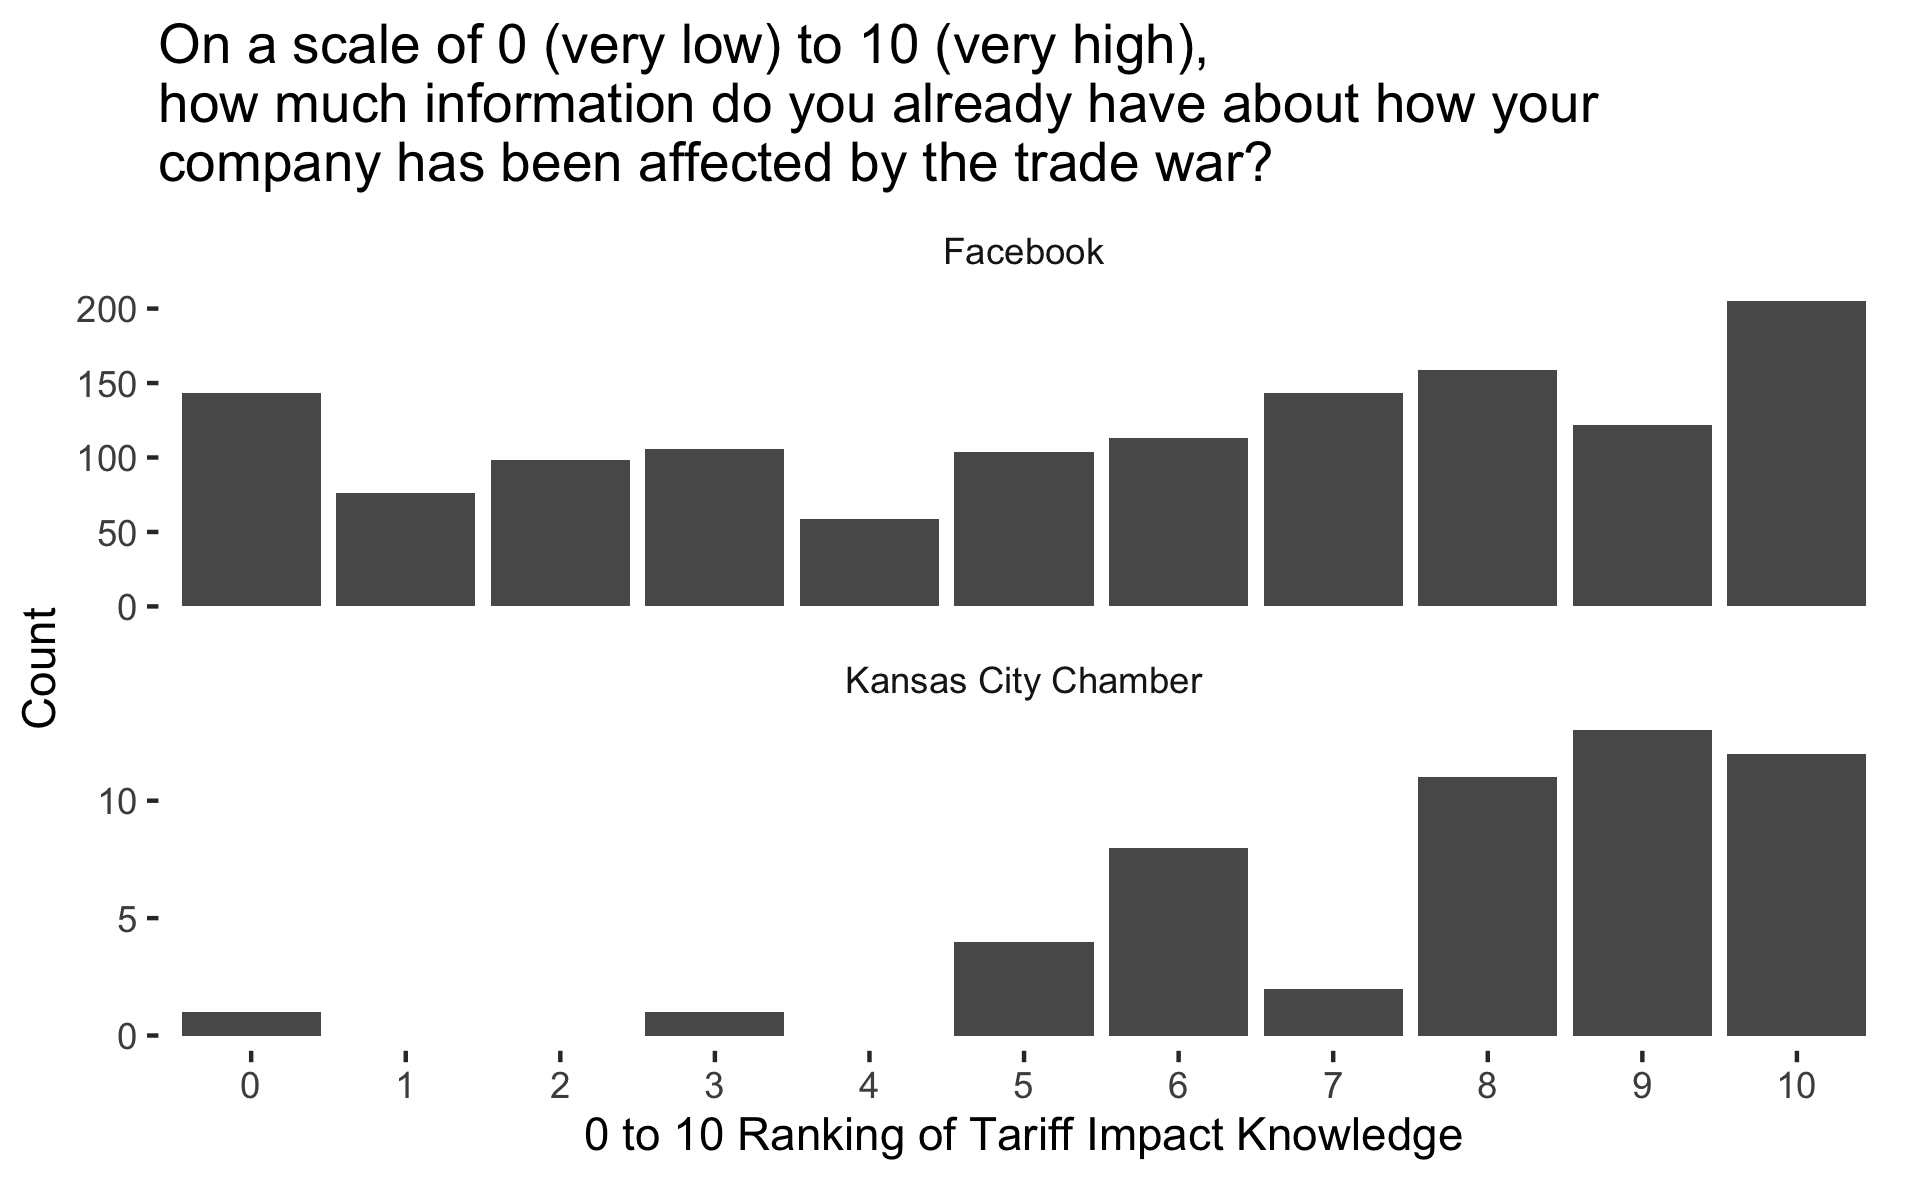
\includegraphics[width=0.7\linewidth]{figures/trade_know.png}
    \caption{Comparison of Facebook and Kansas City Samples for Knowledge about Trade War}
    \label{compknow}
\end{figure}

\begin{figure}
    \centering
    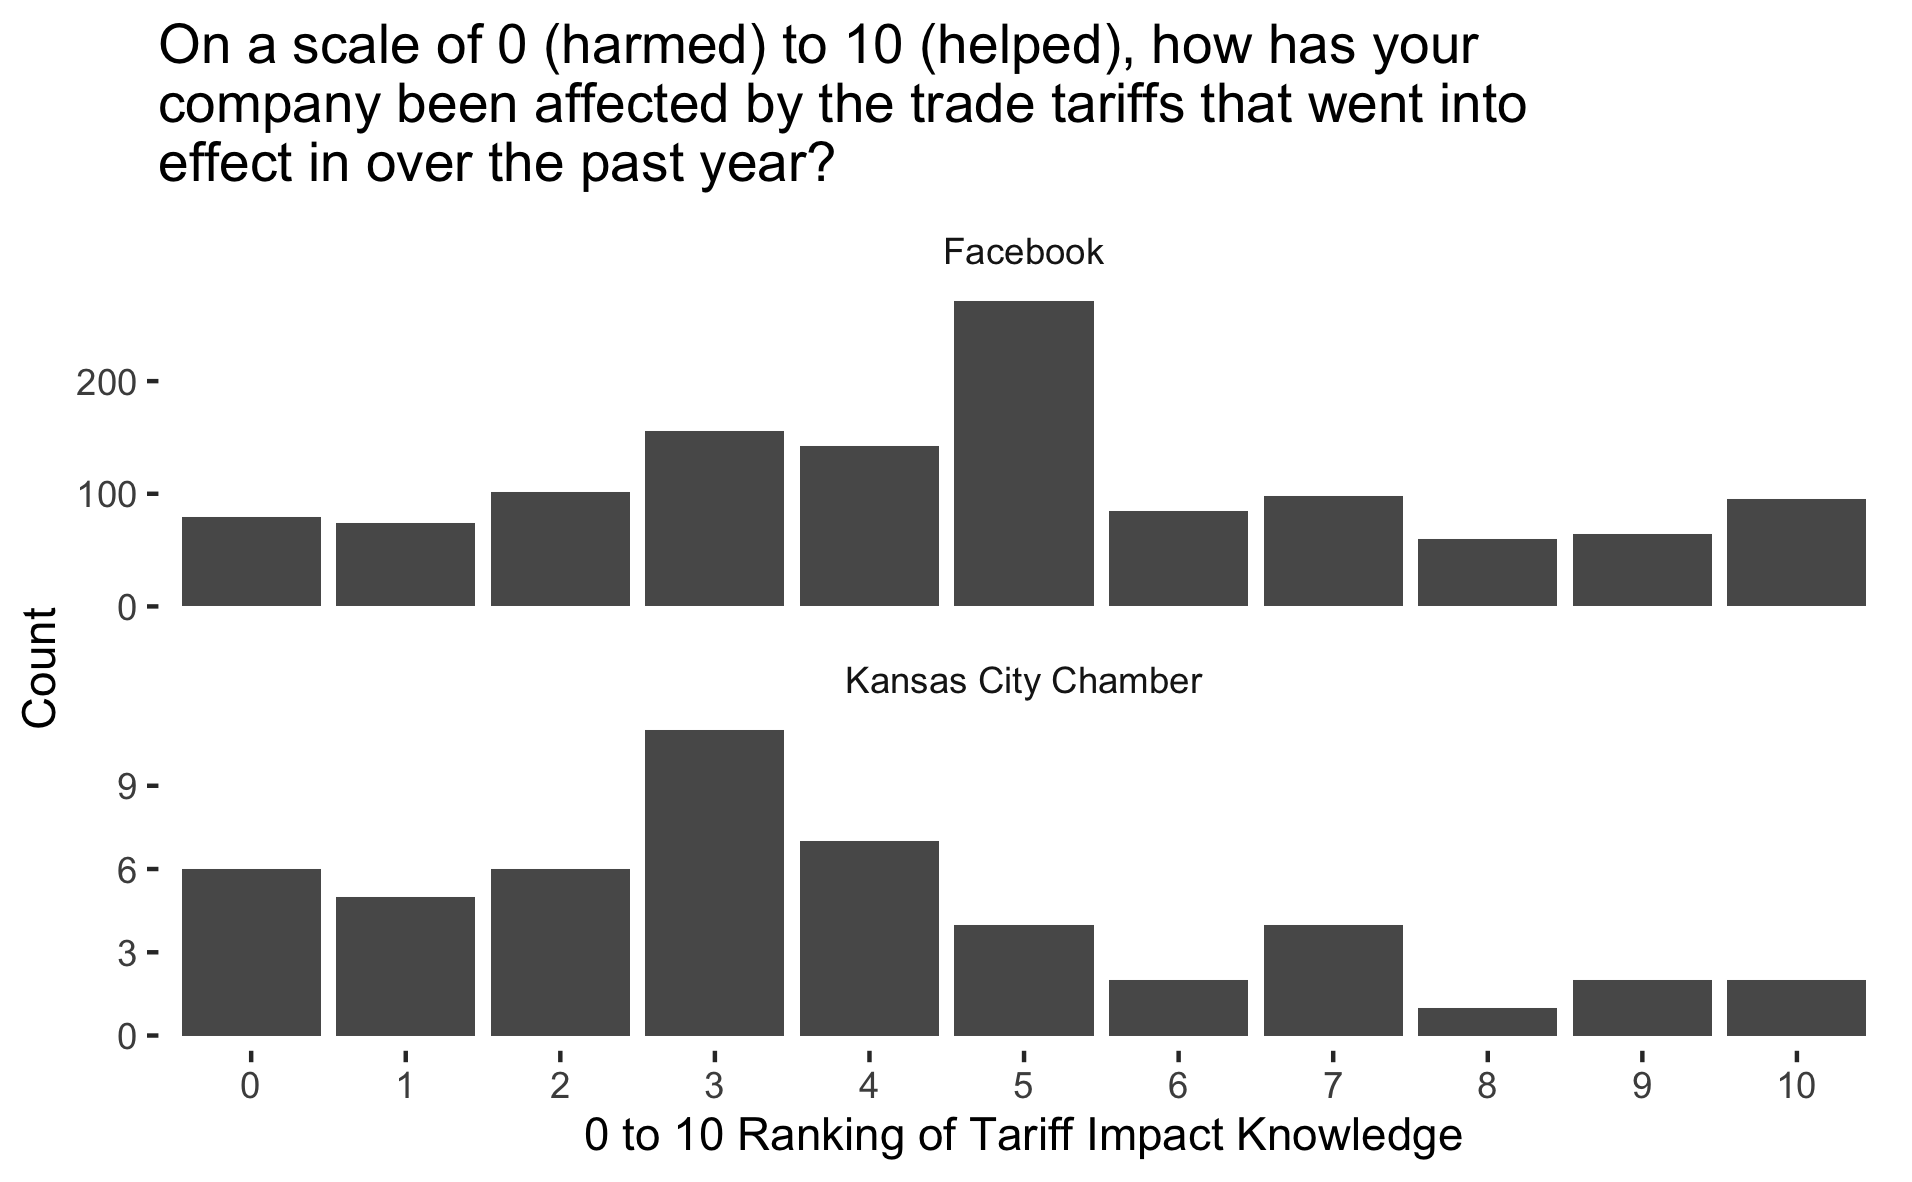
\includegraphics[width=0.7\linewidth]{figures/trade_hurt.png}
    \caption{Comparison of Facebook and Kansas City Samples for Prior Beliefs about Impact of Tariffs on Respondents' Companies}
    \label{comphurt}
\end{figure}

\begin{figure}
    \centering
    \includegraphics[width=0.7\linewidth]{figures/pol_culture_managers_compare.png}
    \caption{Comparison of Facebook and Kansas City Samples for Distribution of Company Managers' Political Ideology}
    \label{comppol}
\end{figure}

In the Appendix, we check the sensitivity of our results to dropping firms with ambiguous companies or industries and a small number of non-managers. Our results are robust.

%We take this over-time variation into consideration in our analysis subsequently.

\subsection{Treatment}

The treatment we provided was information about the impacts of the trade war. We sought to provide a randomly selected group of firms with useful information that would otherwise be unavailable to many of them. Firms would not find a generic estimate of the costs of the trade war on the American economy very helpful; they would want to know how it affected businesses like them. Because of this, we went to great lengths to estimate the costs of the trade war by industry at a highly granular level, and we collected sufficient details from our study participants so that we could provide them with a tailored estimate. We provided firms with the following information: the industries firms like them regularly buy from, the commodities used by those upstream industries, and how many of those commodities faced appeared on tariffs lists.

To be able to provide a precise informational treatment, we needed to (1) estimate the costs of the trade war at a granular level and (2) design a platform to show the correct estimate for a respondent based on their inputs. First, we estimated the costs of the trade war by industry at the NAICS 3-digit level. We made use of input-output data from the Bureau of Economic Analysis, lists of tariffed commodities from the Petersen Institute for International Economics, and a concordance from Pierce and Schott (2009) mapping industries to commodities. We calculate how many goods used by each industry's upstream industries were subject to tariffs. We recognize this estimate is imperfect, but we believe it is much more informative than other figures most small- and medium-sized firms would have seen. The Appendix describes our procedure for estimating these figures in further detail.

Second, we required a platform that would show the correct estimate for a respondent based on their inputs. We used an online survey and collected initial demographic questions --- including the firm's industry --- that determined the information respondents subsequently received. We also randomized how we provided this information. Respondents in the ``static'' treatment were provided with the top six tariff-affected industries to their firm and how many of the commodities used by those industries were tariffed. However, we recognize that an overall industry's inputs do not necessarily map on to an individual firm's inputs. We therefore also developed a ``dynamic'' treatment, in which firms were invited to use an interactive Shiny application that asked them to record the amount their firm purchased from each upstream industry and then calculated how much extra they likely paid in tariffs. While even more precise and informative than the static treatment, we had less control over how participants engaged with it than the static treatment, which we are confident participants receive. We crossed these treatments in a factorial design, so some respondents received both the static and dynamic treatments, while others received no tailored information at all (control).

All respondents, both treatment and control, received the following text:

\begin{quotation}
Please read the following information about the trade war and your company, and then scroll to proceed with the survey. The imposition of tariffs in 2018, recent studies show, cost U.S. consumers and companies \$1.4 billion a month and will force companies to redirect \$165 billion per year worth of imports affected by tariffs. Furthermore, \$121 billion of companies' exports to foreign markets have been harmed by retaliatory tariffs posed by other countries.
\end{quotation}

We included this information in control to ensure that the treatments were not simply a priming effect of reminding respondents about the trade war.

If in the static treatment condition, respondents also received the following text:

\begin{quotation}
``We've crunched some numbers for you. Using data from the Bureau of Economic Analysis, we have identified the most tariff-affected industries that provide important inputs to companies in your industry.''
\end{quotation} 

Participants then saw a list of the six most important industries they input from and, for each industry, the proportion of their products that are subject to tariffs along with the average tariff rate. Firms in the dynamic treatment condition were instead provided with credentials to access the web application. The invitation read:

\begin{quotation}
``We have developed an online application to allow you to calculate precisely how much extra your firm may have paid for goods and services as a result of the tariffs. The application is available exclusively to you because of your participation in our study. You can access the application here.''
\end{quotation} 

%Prior to the treatment, all firms --- both treatment and control --- were told, ``Please read the following information about the trade war and your company, and then scroll to proceed with the survey. The imposition The imposition of tariffs in 2018, recent studies show, cost U.S. consumers and companies \$1.4 billion a month and will force companies to redirect \$165 billion per year worth of imports affected by tariffs. Furthermore, \$121 billion of companies' exports to foreign markets have been harmed by retaliatory tariffs posed by other countries.'' We included these details, which are commonly reported in major news outlets, to provide all firms with an equal understanding of the overall effects of the trade war on the economy. Only our randomly selected treatment group received more specific information through either the static or the dynamic treatment text.

For our main analysis, we collapse the static and dynamic treatments, so we code a 1 for a respondent who has received any treatment and a 0 otherwise. We included both treatments not knowing which mode of delivery would best communicate information, but the mode of delivery was not itself our object of study, so we often combine the two.

Of course, we recognize that the information firms receive varies, and it varies in a way that is systematically correlated with background features of the firm (such as its industry). For the most part, we see this as a strength of our design. \citet{naoi2020survey} critiques many survey experimental tests of support for globalization because their informational treatments---designed to inform the participant about the costs and benefits of various policies---are too general, do not make much of an impact, and trigger sociotropic reasoning. In contrast, our informational treatment is tailored and communicates data we believe our participants would find valuable. Nevertheless, this makes it somewhat more challenging to interpret our data, since each firm receives a different estimate of the trade war's effect. Given the variety in the information we provided to firms, our analysis is most meaningful when it considers heterogeneity in the treatment effect based on the costs we reported to firms.

\subsection{Outcomes}

Following treatment, we measure firms' willingness to take political action. Our strategy is to provide several possible actions they could take and measure firms' interest in each one. We begin by telling respondents that we will present them with a list of actions they can take to support or oppose the tariffs, and we ask which list they would like to see (or both). We do this so that we can distinguish their preference from their willingness to take political action. Our first outcome measure, \textit{Preference}, is whether they seek to see ``Support'', ``Oppose,'' or ``Both.''

Next, we show them the list of actions they requested. Both lists are presented in the following way: ``Here's what you can do to [support/oppose] tariffs. Select any that you are interested in and we will share more detailed information with you on the next page.'' The list of actions appears in Table \ref{tab:outcomes}. We intentionally keep these action items non-specific at this stage, since this allows us to phrase the action items across both lists as similarly as possible. For example, saying ``Donate to Congresspeople who oppose/support tariffs'' avoids mentioning specific legislators who may be especially popular or unpopular. Of course, we provide this detail on the next page when we encourage individuals to actually take the suggested action. We were unable to find a write-in campaign in support of the trade war or governors who publicly supported the trade war, so these action items are missing for tariff supporters. This outcome measure, \textit{Interest}, is closer to measuring political action than \textit{Preference}, but does not necessarily indicate the individual took the proposed action. However, \textit{Interest} is relatively comparable across opponents and supporters of the trade war, given its non-specific framing.

\begin{table}[]
    \caption{Outcome measures}
    \label{tab:outcomes}
    \centering
    \begin{tabular}{p{5cm}|p{5cm}|p{5cm}}
    Interest & Action (oppose) & Action (support) \\
    \hline
      Invite someone to participate in this study & Provides their e-mail address & Provides their e-mail address \\
       Ask your Congressperson to [o] the trade war  & Clicks link to Americans for Free Trade (write-in campaign) & N/A \\
       Donate to governors who [o/s] tariffs & Clicks link to donate to a governor & N/A \\
       Sign a petition [o/s] the trade war & Clicks link to sign petition ``Republicans Fighting Tariffs'' & Clicks link to sign petition from American companies seeking protection \\
       Donate to Congresspeople who [o/s] tariffs & Clinks link to donate to sponsors of Import Tax Relief Act & Clicks link to donate to sponsors of Fair Trade with China Enforcement Act\\
       Join Facebook groups [o/s] the trade war & Likes ``Tariffs Hurt the Heartland'' & Likes ``American Jobs Build America'' \\
    \end{tabular}
\end{table}

Finally, we measure whether the individual actually takes the suggested \textit{Action}. We do so primarily by tracking whether they click the link suggested. Although we are unable to track whether they actually donate or sign after clicking the link, this is the most credible way we have of measuring their behavior. At minimum, clicking the link represents the cost of the individual's (uncompensated) time.

The variety of outcomes we measure helps us to measure political engagement in diverse ways. But in much of our analysis, we collapse these various outcomes. Since we are primarily interested in explaining opposition to the trade war, we operationalize our main outcome measure as a 1 if the respondent showed interest in any political action related to opposing the trade war, and a 0 otherwise. We discuss the support trade war outcome as well where relevant.

\subsection{Estimation Strategy}

We test our hypotheses by estimating the sample average treatment effect (ATE) of providing information and by estimating local ATEs (LATEs) that are conditional on respondents' prior beliefs and the content of the information they were provided. The overall ATE of our treatment tests Hypothesis 1 and measures the overall effect of exposure to information, regardless of the substance of that information. The LATEs help us to test Hypothesis 2, which considers how the effect of information may depend on a firm's vulnerability to tariffs, which they may or may not have been aware of before our treatment. In general, we use logistic regressions to estimate treatment effects with binary outcome variables and we use ordinary least squares (OLS) regressions with count dependent variables.

\section{Results}%https://www.overleaf.com/project/5f0cdef3a8318e0001aa97ca

%Given our several different ways of measuring outcomes, we attempt here to present as diverse an array of analyses as possible for the sake of transparency. Our hypotheses require us to consider both the sample average treatment effects (ATEs) along with local ATEs (LATEs) conditional on pre-existing beliefs and on the number of tariffed products in the respondent's industry. As we noted earlier, our main interest is in explaining opposition to the trade war, and so we present as our main outcome whether a respondent selected a political action related to opposing the trade war. We also consider an aggregated outcome equal to 1 if which a respondent selected any of the oppose trade war outcomes and 0 otherwise. For the treatment, we examine both a collapsed version coded as 1 if a respondent receives any form of the treatment and 0 otherwise, and also separate treatment types (static vs. dynamic versions).  

We found no evidence that the mere act of providing information encouraged firms to oppose the trade war (Hypothesis 1). Table \ref{tab:collapseopp} estimates the overall sample ATE of providing any information in any form. Most of the results are very weak, and for one outcome, the effect is negative (information discouraged firms from acting to oppose).

\input{tables/collapse_opp}

These null findings could be explained if the information was not sufficiently or clearly communicated, but we do not think this is the case either. In Table \ref{tab:allopp}, we separate our static and dynamic treatments to see if there were effects concentrated in one communication strategy. There were not. The strongest effects we observed were for the combination of the two strategies. We suspect this is because our dynamic treatment added credibility to our static treatment, but since relatively few firms engaged with our dynamic treatment, they were more likely to get the necessary information from the static treatment. Regardless of why this combination was the strongest, the effect was to depress rather than encourage political action. Overall, we find no support for our first pre-registered hypothesis. 


\input{tables/all_opp}

%As can be seen, the ATEs are not consistent with our first pre-registered hypothesis. Many of the results show relatively weak effects, and when they are stronger, they are almost always in the negative direction, implying that the simple act of providing a treatment of any kind made it less likely that respondents would take action to oppose the trade war.  

%It is also interesting that the disaggregated treatments in Table \ref{tab:allopp} reveal that the combined dynamic with static treatment had the strongest effect. This combination would make sense if our assumption is correct that respondents are seeking quality information. Providing both an online application and static text should increase the credibility of the information and hence the strength of the treatment.

%However, we do see stronger results for the oppose outcome versus the support outcome results in the appendix, which would be logical as our treatment was aimed at encouraging opposition rather than dampening support

\subsection{Treatment Heterogeneity}

It is perhaps unsurprising that we found null effects of our main treatment: we provided a variety of information to firms with a variety of previously held opinions about the trade war. In this section, we test our more nuanced Hypothesis 2 by investigating the heterogeneity of our treatment effects according to prior beliefs of the trade war's effects. We also consider heterogeneity in terms of the intensity of costs measured by the number of products affected by tariffs across industries.

\subsubsection{Prior Beliefs and Knowledge}

First, we consider how the effects of treatment varied based on firms' prior beliefs about the impacts of the trade war on their business. We measured this by asking respondents to rank on a scale of 0 to 10 how strongly the trade war had either hurt or helped their firm, with higher values indicating that the trade war helped them.\footnote{We stress that this indicates the respondent's perception of the trade war's impact, not necessarily the reality of their firm's experience. Nevertheless, perception is what matters for a firm's decision-making.} As we showed in Figure \ref{comphurt}, prior beliefs varied widely in our sample. In the Appendix, we explore the determinants of these prior beliefs descriptively, but here we focus on how they condition our experimental treatment effects. In Hypothesis 2, we expected that our information would have the strongest effects for those firms who felt neither especially helped nor hurt by the trade war; firms on either extreme end of the scale would have already found it in their interest to seek the kind of information we provide.

We find evidence to support this. Figure \ref{hurtknow} presents the LATEs of receiving any of our treatments on taking any action to oppose the trade war for each level of respondents' prior beliefs about the trade war's impact (model results are available in the appendix). This figure is our cleanest test of our second hypothesis regarding pre-existing beliefs. We find this hypothesis to be partially supported and partially falsified. First, we do note a distinct quadratic relationship, as we hypothesized: the strongest effects exist for those with middling prior beliefs. However, the  empirical relationship is convex, not concave, meaning that the effects for this group were most negative, not most positive. This difference in what we expected may help explain why we also find overall negative effects of the trade war: respondents with limited information about the trade war may have been convinced a priori that its effects were worse than they in fact turned out to be, so this information discouraged them from opposing. However, as we noted in the discussion of our model, there are several other factors that need to be taken into account in terms of how respondents were likely to interpret the treatment.

%In theory, this relationship should be linear and negative: the more a respondent believes they have been helped by the trade war (10), the less likely they should be to take action to oppose it. In both treatment and control conditions, we do observe that those who perceived they were very harmed by the trade war are more likely to take action to oppose it (about 25-35\%) than those who perceived they were helped (about 10-20\%). But in control, the relationship is not at all linear: control respondents with a moderate perception of harm from the trade war are more, not less, likely to oppose the trade war than those who believe they have been greatly harmed. Our informational treatment, however, restores the logical linear relationship. We interpret this as evidence that providing individuals with information about the impacts of the trade war causes them to take political actions that are logically consistent with their prior perceived interests. The treatment especially influences the behavior of those firms without extreme priors about the impacts of the trade war who perhaps did not consider it worthwhile to learn more about the trade war's impacts. We also observe that the treatment encourages firms at both extremes to oppose the trade war. Respondents who already felt themselves to be harmed by the trade war may have been goaded into taking action, while those who felt themselves to be helped perhaps learned information that conflicted with their beliefs and changed their minds, becoming less likely to take action supporting the tariffs.

%We investigate this more systematically in the Appendix by calculating LATEs for each value of our prior belief scale. Specifically, we interact the treatment with each value. The results confirm that the above differences are significant, but we focus on predicted probabilities in the main text for ease of interpretation.

%As can be seen in Table \ref{hurtknow}, in control, or in a situation in which the respondent does not receive any information pertinent to their firm, opposition to the trade war is in fact highest for companies in the middle of the distribution, i.e., those who appear to be uncertain as to whether the trade war helped or hurt them. This comports with our minimalist formal model because those who \emph{did not} receive the treatment are highly conditioned by pre-existing beliefs. Those firms which lack information about the trade war are also presumably those which are most curious about political opportunities as they presumably did not consider it rational previously to make the investment to learn about  the trade war.

%It is important too to note that the second highest group in control are those who had pre-existing beliefs that the trade war was very harmful. These firms of course stood to gain from opposing the trade war; their rates of participation may be lower than the uncertain group because they may have already researched and taken political action. However, they are still significantly more likely to oppose the trade war (approximately 25\%) relative to those who believed the trade war was very helpful (approximately 15\%). 

%The treatment distribution, on the other hand, slopes monotonically downwards as we might expect in a world in which companies have perfect information about tariff costs. In essence, the treatment is overcoming uncertainty and inaccurate information about the trade war's potential benefits relative to control. In treatment, those who thought the trade war had harmed them are now the most likely to oppose the trade war, though their rate of participation is roughly similar to the rate in control. On the other hand, those who thought the trade war helped them became modestly more likely to take action opposing the trade war, possibly because the information about tariffs conflicted with their prior inaccurate beliefs.

\begin{figure}
    \centering
    \includegraphics[width=0.7\linewidth]{figures/treat_hurt_trade.png}
    
    \raggedright \scriptsize Plot shows LATEs for the opposing trade war outcome conditional on the respondents' answers to the question,``On a scale of 1 to 10, has the trade war helped or hurt your firm?". The dependent variable is a 1 if the respondent selected any action to oppose the trade war, 0 otherwise. Treatment is a 1 if the respondent received any treatment, 0 otherwise.
    \caption{LATEs for Opposing Trade War by Prior Beliefs about Trade War}\label{hurtknow}
\end{figure}

%This complexity in treatment heterogeneity suggests why it might be difficult to detect useful ATEs. The effect of the treatment appears to be strongly influenced by firm-level heterogeneity. However, we note that beliefs about the trade war's efficacy does not directly address the amount of information available to these companies prior to observing the treatment.

One important consideration is that the impact of our treatment may have depended not only on the prior beliefs held by respondents but also on how well informed those prior beliefs were. For this reason, we next investigate treatment heterogeneity based on the joint association of prior beliefs and prior knowledge about the trade war.\footnote{See the Appendix for descriptive analysis of managers' self-assessed knowledge.} We measure prior knowledge similarly to prior beliefs by asking respondents to rank on a 0 to 10 scale how much knowledge they had about the trade war. As we showed in Figure \ref{compknow}, prior knowledge varied widely in our sample (with the Kansas City sample being significantly more knowledgeable than the Facebook sample). To estimate our results, we fit a logistic regression model with a collapsed treatment variable and a three-way interaction between the treatment (0-1), the prior beliefs variable (0-10), and the prior knowledge variable (0-10). We plot the results as LATEs on opposing the trade war for the entire joint distribution of the two pre-treatment covariates in Figure \ref{fulldist}. The model results are available in the appendix. 

A straightforward result from this analysis is that we observe the strongest treatment effects for low information respondents, and these respondents reacted in ways that were consistent with their prior beliefs though not necessarily with the treatment. Low-information respondents who believed they were hurt by the trade war became more likely to oppose, while low-information respondents who believed they were helped by the trade war became less likely to oppose, as a result of our treatment. In other words, the treatment backfired for low-information respondents who believed the trade war was helpful. Our informational treatment is less effective for higher-information respondents, as we surmised due to the fact they already had information about the trade war, though there is no sign of respondents reacting adversely to the treatment. Those who had information about the trade war and believed it was helpful became more likely to consider opposing it once they received our information, as we would expect. Finally, we stress that this joint distribution is stretching what we can obtain with our data, and only the corners of Figure \ref{fulldist} are statistically significant at conventional levels ($p=0.1$). We cannot make clear inferences about what is precisely happening in the middle of the distribution.

%Our logic for Hypothesis 2 states that respondents who perceived they were neither strongly helped nor hurt by the trade war had less incentive to obtain information, which is why our treatment would have the strongest effects for them. If this is the case, we would generally expect our treatment to matter least for those with high prior knowledge and most for those with low prior knowledge, although it may impact firms differently within these groups based on their prior beliefs.

%We find evidence consistent with this thinking. The control group can be distinguished as high-information (rational) behavior versus low-information (irrational) behavior. The top part of the control plot in Figure \ref{fulldist} shows expected perfect information behavior: those who believed the trade war hurt them and had a lot of evidence to prove it, were more likely to oppose the trade war (more than 50\%). Conversely, those who knew a lot about the trade war and believed it was helpful to their company were unlikely to oppose it (less than 10\%). 

%By comparison, the low-information part of the control plot (i.e., the lower half) reveals seemingly irrational behavior. Those who believed the trade war helped them are less likely to select an opposition outcome, while those who believed the trade war would harm them are in fact more likely to do so. %This puzzling phenomenon aligns with our theory: those who do not have adequate information to make decisions may not take actions that are consistent with their perceived interests.

In essence, we can see that the treatment's effects were highly mitigated by low-information beliefs. Those who had strong beliefs about the trade war and who had high levels of information remained likely or unlikely to oppose the trade war based on their own prior beliefs, leaving less room for the treatment to work, though when the treatment worked, it did so as we would expect. By comparison, for those in the low-information group, the treatment had effects that went in accord with prior beliefs even if it meant the opposite of what our treatment provided: for those who believed the trade war helped them, the treatment increased their willingness to oppose the trade war. In other words, respondents who rated their own level of knowledge about the trade war as poor relied more on their prior beliefs when deciding whether to take action. On the other hand, those who had a high level of knowledge were relatively unmoved by information provided by the trade war but did so in a way we would classify as strictly rational given our model. 

\begin{figure}
    \centering
    \includegraphics[width=0.7\linewidth]{figures/both_know_hurt_trade.png}
    
    \raggedright \scriptsize Plot shows LATEs for the opposing trade war outcome conditional on the respondents' answers to the question,``On a scale of 1 to 10, has the trade war helped or hurt your firm?" and the question, ``On a scale of 1 to 10, how much knowledge do you have about the trade war?". The dependent variable is a 1 if the respondent selected any action to oppose the trade war, 0 otherwise. Treatment is a 1 if the respondent received any treatment, 0 otherwise.
    \caption{LATEs for Opposing Trade War by Prior Beliefs and Knowledge about Trade War}
    \label{fulldist}
\end{figure}

In summary, we can say that these results support our theoretical expectations about the role played by prior beliefs and knowledge. However, our second hypothesis proved to be too simple as it supposed that we could see a clear bivariate pattern when beliefs and knowledge tend to interact with each other. To gain insight into how the treatment affected respondents, we needed to examine both of these factors jointly.

So far, we have shown that information about the trade war mattered most to firms who previously believed they were neither helped nor hurt by the trade war and to firms who assessed their previous knowledge of the trade war as poor. However, we have made the assumption so far that the treatment provided a similar level of information to companies conditional on beliefs, when in fact the treatment varied by industry. In the next section, we consider the role played by the actual content of the tailored information we provided to firms to obtain a more complete picture of the treatment's effects.

\subsubsection{Content of Information}

What we have left out of the analysis so far is the fact that respondents received different information depending on the number of products in their industry that were affected by tariffs. Some firms were informed they faced extensive costs, while others faced relatively few. In this section, we estimate the effect of information conditional on the content of that information. Since the content of information is not randomly assigned, we calculate LATEs, conditional on the content of the information respondents were (or would have been) shown.

We summarize the content of the information shown to respondents by calculating the number of products with at least one tariff that were shown to the respondent. We considered other possible summary statistics: the average tariff rate for all input products, the total number of products with tariffs and the average proportion of products across the respondent's input industries with a tariff of any kind. In the end, all these variables were highly correlated from .7 to .9, and we selected the number of products with tariffs because its distribution had considerable variation and desirable properties. We illustrate this distribution in Figure \ref{histtreat}, and the distribution is balanced between treatment and control. There were many respondents who were in industries utilizing over 1000 products on tariff lists, and those in treatment were informed of this. There were also several respondents in relatively unaffected industries. The pronounced mode at zero includes respondents who did not match any products.\footnote{Some respondents (8\%) were in NAICS codes for which we could not identify any input products which had tariffs. Some of these may be due to limitations in the coverage of the BLS input-output tables.} In the Appendix, we show that a respondent's prior beliefs significantly predicts the number of products we showed (or would have showed) them. We interpret this as reassuring evidence that we and our respondents more often agreed than disagreed about the effects of the trade war on their firm.

\begin{figure}
    \centering
    \includegraphics[width=0.7\linewidth]{figures/treathist.png}
    \caption{Histogram of Respondent's Industry Products with Tariffs}
    \label{histtreat}
\end{figure}

%We expect the content of the information to interact with the respondent's prior beliefs about the impact of the trade war. To model this, we borrow from the idea of treatment ``dosage'' in medicine \citep{prentice_generalization_1976} and try to make the treatment proportional to each respondent's vulnerability to the treatment. We believe the best way to do so is to divide the number of tariffed products shown by the respondent's prior belief (0 -- hurt -- to 10 -- helped) --- this too is an interaction term, but using division rather than multiplication allows the impact of number of products to be proportional to a respondent's prior beliefs. The more products receiving tariffs, the higher this value; the greater the prior belief that the trade war helped, the lower this value. We subtract away the midpoint of the scale so that we have instead a range of -5 to +5, which permits us to allow 0 to signal that the respondent does not have prior beliefs that would bias them one way or another. For the product scale, we further recode any zeroes in the treatment condition to the minimum value of products times -1 so that we can model the fact that those in the control condition in fact received more dosage than those in treatment who were informed that no products in their industry had tariffs. While our hypotheses primarily center on opposition to the trade war, for this analysis, we also consider whether firms might take action to support the trade war, as this information may lead them to update in either direction.

%We find that the content of the information we provide, proportional to prior beliefs, is strongly associated with the probability of taking action, but in the opposite direction of what we would expect. The complete results appear in the appendix in Tables 4 and 5, which report the coefficients of our main interaction term, Products / Prior Beliefs (Hurt). As can be seen, there are quite strong associations between this adjusted product score and outcomes opposing  and supporting the trade war, though the results are more consistent for supporting the trade war. However, we note that the aggregate outcome (Any) for opposing the trade war shows a clear association, and the count of opposition outcomes model has a reasonably strong association ($p=0.11$).  

%In Tables \ref{intoppose} and \ref{intsupp} we show the results of interactions between the count of products shown and respondent beliefs about the trade war for both the oppose and support trade war outcomes. In addition to the any selected outcome, we also include a count outcome for the total number of clicks on political options by respondents. We show both support and oppose outcomes in this analysis as treatment dosage could affect either even if our hypotheses primarily center on trade war opposition. 

%While the results show that there are clear effects of the adjusted product total shown to respondents, it is difficult to understand the results substantively without plotting the change in outcomes. In Figure \ref{treatstrength} by calculating the sample-average predicted value of taking any action to support or oppose the trade war given a grid of the possible values for the number of products shown to respondents and their prior belief about the effects of the trade war. While the two plots may look like mirror images, they in fact communicate quite different stories.

Figure \ref{treatstrength} presents the LATEs for both the oppose and support trade war outcomes. First, we consider actions taken to oppose the trade war.
%On the whole, it would appear that tariffs here interacted with beliefs in a positive direction; i.e., the more respondents thought they had been hurt by. the trade war, the more they were willing to oppose the trade war.
Among respondents who held a prior belief that they had been very hurt by the trade war, there was a very logical relationship between the information we provided and their willingness to oppose the trade war: the more tariffs they faced, the greater impact our treatment had on their willingness to take action. They may have been willing to take action to oppose the trade war on their own, but their opposition grew significantly as a result of receiving our information. 
We do not see as strong or clear patterns for those who believed the trade war would help them.
%The treatment differences between low and high numbers of tariffs are smaller, though it would appear that there is a tendency for increasing numbers of tariffs to further reduce interest in opposing the trade war.
In addition, it appears our treatment yet again backfires for those who believe they are neither helped nor hurt, or weakly helped, by the trade war.
For these respondents, the more tariffs they faced, the more our information dissuaded them from taking action to support the trade war. In other words, for those who had countervailing beliefs to the treatment, showing them more and more products resulted in increasing resistance to the treatment.
%This is the first example we have seen of this type of behavior, i.e., the treatment producing the opposite effect of what we might expect.

These results were, of course, not predicted and remain puzzling. It appears that an important set of subjects were confronted with information that contradicted their priors. We expected that such subjects would update to the information and act according to their interests. Instead, they appear to behave opposite to their interest and to our predictions. We discuss some possible explanations at the end of this section.
%We can only speculate as to why. One possibility is that these subjects were preemptively and strategically reacting to the information to counteract the political action of other subjects whose resolve to oppose the trade war might have strengthened after receiving the treatment information. But this is mere speculation. Another possibility is simple backfire in the face of information that contradicted a firmly held prior.  

Second, we consider actions taken to support the trade war. We note first that we are displaying this outcome because we want to understand the effect of showing varying numbers of tariffs: our theory and treatment has less to say about support for the trade war than it does about opposition. First, among respondents who held a prior belief that they had very much been helped by the trade war, there was a straightforward relationship between the information we provided and their willingness to support the trade war: the more tariffs they faced, the more our information deterred them from supporting the trade war. For the rest of the plot, however, we do not see large differences in the size of the treatment effect from showing varying numbers of tariffs. Respondents who received the treatment were modestly more likely to support the trade war, but the estimated effect is close to zero, and it does not appear to vary significantly based on the number of tariffs that were displayed. As such it does not appear that respondents internalized the content of our information in a way that changed their support for the trade war, aside from those who previously held strong beliefs that the trade had helped their company.

\begin{figure}
    \centering
    \includegraphics[width=0.7\linewidth]{figures/strength_treat.png}
    
    \raggedright \scriptsize Plot shows LATEs for the opposing trade war and supporting trade war outcomes given the number of tariffs displayed to a respondent in the treatment and subset by the respondents' answers to the question,``On a scale of 1 to 10, has the trade war helped or hurt your firm?" The dependent variable is a 1 if the respondent selected any action to support/oppose the trade war, 0 otherwise. 
    \caption{LATEs for Opposing and Supporting Trade War by Content of Information and Prior Beliefs}
    \label{treatstrength}
\end{figure}

%There are two possible explanations for this perplexing finding. The first is that because these respondents believed the trade war had helped their firm, learning that relatively few products had tariffs led them to conclude that the trade war benefited them less than they had supposed, making them less likely to take action. However, there are some problems with this explanation, notably that we exposed respondents to tariffs on their industries' inputs, not on goods they might sell for which they could reap above-market profits. In addition, we do not observe the opposite relationship among those who believed the trade war hurt their company: their willingness to take action supporting the trade war is not at all related to the number of tariffed products they saw. Finally, companies that benefited from the trade war received quite strong protection from competitors and it is unlikely our purely informational treatment could move them into the opposition category.

A takeaway is that higher levels of the informational treatment do appear to have caused two groups to change their behaviors in an anti-tariff direction. First, the treatment had an effect for those who incorrectly believed they were helped by the trade war, but were in fact heavily hurt. This group was receptive to the increasingly concerning information we provided and became less likely to support the trade war (although they did not become significantly more likely to oppose it). Second, it worked for those who correctly believed they were hurt by the trade war. Within this group, those who received our informational treatment were significantly more likely to take action to oppose the trade war. Perhaps the information they received provided them with the evidence they required to push them to action.

But for some respondents --- especially those without strong convictions about the trade war --- our informational treatment counterintuitively moved respondents in a pro-tariff direction. Informing managers who did not think the trade war impacted them much that they in fact faced thousands of tariffs caused those managers to be less, not more likely to oppose the trade war. One possible explanation is that we observe backlash to counter-attitudinal information in our imperfectly rational respondents. While we can't rule this explanation out, we note that the existing evidence for this theory is mixed \citep{guess2020does}. If it did occur, it likely is related to the role of ideological views within companies, as we discuss in the next section.

An explanation anchored in collective action theories is that our treatment, which was primarily intended to improve awareness of the benefits of collective action, also affected respondents' beliefs about the probability of success. While respondents who saw more tariffs affecting their industry would enjoy greater benefits as a result of ending the trade war, they may have also become overwhelmed by the enormity of the problem, which could discourage them from taking action. We tried to prevent this by providing a general statement about the massive size of the trade war to everyone --- both treatment and control --- so that all participants would have an equally daunting sense of the challenge of reversing these trade policies. But it is possible that that the respondents who saw many tariffs affecting their business were more likely to conclude that the trade war would be too difficult to end, so the probability of obtaining these benefits would be lowered.

But our preferred explanation hinges on the idea that many firms supported the trade war for principled reasons. Several managers expressed in open-ended comments that they felt the trade war would benefit the U.S. economy in the long run, even if it hurt their business today. When these respondents saw the price firms like them were paying (and that we were publicizing it), they may have grown concerned that others would bail, and instead doubled-down on their support for the trade war. This explanation imagines that there is also a collective action problem associated with support for the trade war, since firms believe they must  endure costly tariffs to promote the success of the U.S. economy. Our treatment may have signaled to the most principled of these firms that their peers might cave, causing them to increase their support to prevent growing opposition. Critically, this explanation requires some firms to support the trade war despite being aware of its costs. While we cannot rule out alternative explanations, we believe this one comports with our data. In the next section, we provide preliminary evidence that managers hold these kinds of ideological beliefs.

Finally, we note that it is difficult to examine LATEs by more than two variables. As we described earlier, the level of knowledge about the trade war can have implications for how prior beliefs interact with the treatment. However, including that variable would require examination of a three-dimensional response surface that would be difficult to describe, let alone integrate into our theoretical conclusions. We believe it may be necessary for future experiments to more closely pin down the interaction between strength of treatment, extent of prior knowledge and type of prior knowledge. 
 
\subsection{Political Culture}

Our final set of findings relate to a relationship with opposition to the trade war that we did not discuss in our pre-registration --- though of course in hindsight it now it appears obvious --- that of the role of political ideology.\footnote{We primarily use the term ``political culture'' because this is the term we used with survey respondents. We interpret their responses, which range from very liberal to very conservative, as an indicator of the ideological beliefs that predominate in their companies. We did not ask about party affiliation, but we suspect these ideological views are polarized along partisan lines.} Because we asked respondents about the ``political culture'' of their companies both among management and rank-and-file we can consider the relationship between these variables and willingness to oppose the trade war. While we asked managers to characterize the political identities of their companies, not themselves, we realize their responses may well reflect their personal views, and take our findings with a grain of salt. Again, since political culture is not randomly assigned, we underscore that these results have no causal interpretation.

We find that political culture is an extremely strong predictor of a firm's decision to oppose the trade war. Figure \ref{polman} reports probabilities of opposing the trade war for each level of a firm's political identity. The relationship is extremely strong, even considering the level of polarization during the Trump presidency. Those who reported working at a very conservative firm had a probability of selecting an opposition outcome of only 10\%, while half of those who worked at liberal or very liberal companies selected an opposition outcome. While this pattern makes sense given current politics, we note that it is a historical departure, as left-leaning companies used to support trade restrictions that would prefer American workers. One takeaway from these findings is that political views may play an important role in explaining prior beliefs about the trade war and, consequently, the strong associations we see between these beliefs and the effect of the treatment.

\begin{figure}
    \centering
    \includegraphics[width=\linewidth]{figures/politics_trade.png}
    
    \raggedright \scriptsize Plot shows the survey proportion selecting at least one opposition to the trade war outcome subset by the political culture of the firm reported by the respondent for both management and rank-and-file employees in the company. The dependent variable is a 1 if the respondent selected any action to oppose the trade war, 0 otherwise. 
    \caption{Role of Political Culture in Explaining Opposition to Trade War}
    \label{polman}
\end{figure}

While these findings are observational, the magnitude of these ideological effects is far stronger than any informational treatment we provided to firms, even though our information did have some impact. We suspect that firm behavior is heavily shaped by the political views held by their employees and managers. If true, this would supply an alternative explanation for \citet{zhu2021firms}'s finding that firms in Republican districts are less likely to oppose the trade war. While they suggest this is for fear of political backlash from their consumers, it may be that managers of those firms are more likely to lean Republican and base their assessment of costs and benefits on their partisan beliefs. Our evidence can't adjudicate between these two explanations, but the strong patterns we observed at the level of the firm's individual political culture --- and not just the partisanship of the district --- suggest this matters. The cost-benefit calculation firms engage in may not be strictly rational.

\section{Discussion}

We believe that our findings shed light on previously poorly understood dynamics about how companies make decisions about whether to push back against trade wars. While much is known about the companies that benefit from trade actions, our study shows in much more detail how companies whose benefit or harm is more tenuous react to more detailed information about how the trade war has likely affected them. As is obvious in retrospect, we did not find an overall average treatment effect across our sample (as we predicted in Hypothesis 1). Instead, we found local average treatment effects concentrated in particular groups of firms, depending on their prior beliefs and knowledge about the trade war as well as the content of the information we provided them.

At first glance, our informational treatment rationalized the relationship between a firm's prior belief and their willingness to take action to oppose the trade war--at least for companies with strong prior beliefs. Logically, firms should be more likely to oppose the trade war the more they sense the trade war has hurt them. Consistent with our theory, we take this as evidence that information is what some firms needed to act on their intuitions, but lacked the motivation to seek out. Similarly, we found that providing information eliminated irrational support for the trade war among some firms with poor prior knowledge of the trade war--at least if these firms' prior was that the trade was harmful. All of this evidence is consistent with Hypothesis 2, that the strongest treatment effects would occur for firms with middling beliefs about the impact of the trade war, who did not care enough about the issue to invest in obtaining information. Once obtained, though, information caused them to act in line with their prior beliefs about the impact of the trade war in ways that we did not anticipate.

When we analyzed the role played by the content of the information we provided, we saw a similar story. Those very same respondents --- those with middling beliefs about the impact of the trade war --- responded to our information, but they responded in counterintuitive ways. If their firm faced thousands of tariffs, informing them of this made them less rather than more likely to oppose the trade war. We observed more logical reactions to the information our treatment provided among the firms with strong prior beliefs that the trade war helped or hurt them. For both these groups, our information moved firms in a more anti-tariff direction the more tariffs they faced.

We believe that firms who were genuinely helped or hurt by the trade war know who they are and take political actions in line with their business's interests and with the content of the information they receive. Firms without strongly informed prior beliefs about the impacts of the trade war on their firm are probably less individually affected by the trade war. But this does not preclude them from having political opinions about the trade war or from taking action. For instance, some managers left open-ended comments indicating that the trade war was the right thing for the American economy, and they would support it even if their business had to pay in the short-term. Among these businesses, our information may have unintended effects. Managers may have grown concerned about other businesses' willingness to stick out the trade war and become less likely to take any action that would oppose it.

On the whole, our results show that credible and detailed information has the potential to rationalize the behaviors of firms, but we underestimated the importance of the role played by political convictions and poorly-informed yet strongly held beliefs about. the trade war. Our analysis of political ideology reinforced this. Companies with liberal cultures are much more likely to oppose the trade war than companies with conservative cultures. Although this finding is not experimental, and therefore not causal, we could not have measured this relationship but for fielding a survey to U.S. business managers, and it suggests these small firms may behave more like individuals than like larger firms when it comes to taking political action. Rising political polarization in the U.S. has been shown to predict countless political and even non-political attitudes, including health behaviors during the COVID-19 pandemic \citep{mccarty2016polarized,gadarian2021partisanship}. We show that political views affect how businesses conceive of their interests. Our work joins a growing literature emphasizing the importance of employees' political attitudes in business activity \citep{duchin2021political}.

Taken together, these results suggest a number of critiques for the collective action model we proposed. On the one hand, we did find evidence in support of Hypothesis 2: information mattered most for firms without strong prior beliefs about the trade war. But when we examined how those firms reacted to the substance of that information, we learned that they did not use that information to act on the interests of their business, as we had assumed they would. Our collective action model did not account for the possibility that firms would value sociotropic interests that reflected their political views. Firms who supported the trade war may also have counter-mobilized to the collective action we were trying to encourage. While information can motivate some businesses to take action in the way our model expected, for other firms, it may backfire.

A scope condition for our study is that respondents may not have viewed the information we received as credible. We sought to make our information credible by branding ourselves with an official-looking website and disavowing any partisan ties. In the end, we believe the element that made our information most credible was our development of an app, since the treatment effects were stronger for this condition despite limited user engagement with the platform. Nevertheless, respondents may not believe our information or may have viewed it as politically biased, as our survey took place during a period of intense political polarization. This could mean that our treatment effects are underestimated.

We also reiterate that our results pertain to small and medium-sized businesses. We believe that recruiting this subject population helps expand the scope of theories explaining trade actions, but these same dynamics are unlikely to hold for very large companies with substantial existing investments in lobbying and other types of political action.

\section{Conclusion}

Trade wars occur in information-scarce environments. Complex global supply chains both exaggerate the economic consequences of a trade war but also complicate firms' abilities to accurately assess this. This is especially true for small and medium-sized firms. Small and medium-sized firms lack the analytical capacity of multinational corporations. They may not experience the effects of a global trade shock in the same ways, but they still likely face higher input costs, whether or not they know why. They may not participate in national politics as Apple does, but their managers and employees can still contact their representatives and vote, whether or not they will. These firms face a classic collective action problem: while they would all benefit through political mobilization, they lack even the information to know whether the costs of seeking information are worth paying.

Providing firms with information about how they are impacted by tariffs should, in theory, help them to solve this collective action problem. We tested this claim through an innovative field experiment in which we provided approximately 1,000 business managers with tailored, high-quality information about the tariffs that impacted their firm. Although our informational treatment provided the evidence some managers needed to oppose the trade war, it had the opposite effect on other managers. By exploring the heterogeneity of our treatment effects based on managers' prior beliefs and knowledge about the trade war, and the content of the information each firm received, we learned that the collective action model suffers from some limitations. Specifically, it omits the possibility that businesses, like individuals, can take action based on sociotropic interests tied to their political beliefs, or that efforts to encourage collective action could elicit counter-mobilization.

In short, we do conclude that businesses face a collective action problem when opposing a trade war, but they also face additional hurdles. Information does help many firms to take actions that are in line with their prior beliefs and the interests of their firms. But the counter-intuitive effects of information on other firms suggest that solving the collective action problem is not sufficient. Further, efforts to solve the collective action problem among sympathetic businesses may make the other barriers to opposition worse. In this way, a main implication of our study is that canonical theories of collective action may be of limited utility in environments of political polarization.

A second implication of our study is that small and medium-sized businesses may have more similarities to individuals than previously thought. We demonstrate that these firms are not always rational actors who take profit-oriented decisions. Like individuals, they have political cultures that inform their beliefs about what is in their and the national interest, and they take political actions that reflect those cultures. We believe that political action among small and medium-sized businesses remains an underexplored area of study.

Finally, our study implies that trade wars are harder to politically oppose than previously thought. Businesses should be the main opponents of a trade war in a world with complex supply chains. But in a world with political polarization, they may be less likely to act on those interests, or may perceive them through ideological lenses. While trade wars have historically been unpopular, increasing political polarization may make them more tolerable among ideologically sympathetic firms.

\newpage
 \setcounter{page}{1}
 \pagenumbering{arabic}

\bibliographystyle{AJPS}
\bibliography{References}

\newpage 

%\KOMAoptions{paper=landscape,pagesize}
\recalctypearea

\Large \textbf{\center{Appendix}} \normalsize
\raggedright

%\setcounter{page}{1}
%\renewcommand{\thepage}{A\arabic{page}}

\setcounter{figure}{0}
\renewcommand{\thefigure}{A\arabic{figure}}

\setcounter{table}{0}
\renewcommand{\thetable}{A\arabic{table}}

\setcounter{section}{0}

\section{Facebook vs Non-Facebook Sampling}
\subsection{Outreach via Web Scraping Emails}
We employed several different strategies to recruit companies to obtain a diverse and representative sample of managers. We found some methods, particularly targeted Facebook ads, to be far more effective than others. As discussed in our pre-registration, our initial sampling strategy involved collecting a substantial number of email addresses of a cross-section of U.S. firms. We were interested in hearing from all firms and not just the larger publicly-traded companies with established government relations practices. To do so, we began with a random sample of all U.S. firms in the Orbis database, and then used web crawling techniques to identify email addresses. Orbis data reflects the pattern of business establishment in the U.S., meaning that the vast majority of firms represented are small (under 5 employees) and concentrated in the services sector (ex. retail, professional services, transportation, leisure and hospitality etc). This sample is appropriate because firms of all sizes and all along the supply chain, including non-tradable firms, could potentially experience tariffs if they use any tradable input. For example, housing construction is non-tradable but the steel, aluminum, and lumber used are exposed to tariffs. 

However, we found this sampling method to be impractical because of aggressive spam filters and the deluge of questionable emails that business managers receive. For this initial wave during June 2019, we reached out to over 12,000 firms by email and only received 2 survey responses or 0.017 percent. Many of the emails generated by web crawling were general inquiry info@companyname.com rather than personal email addresses. After sending out a reminder email and receiving more angry requests to stop spamming respondents than actual survey responses, we changed our outreach strategy. 
\subsection{Outreach via Phone and Email}
From August 2019 to March 2020, we assigned research assistants to manually look up the emails and phone numbers of managers, introduce the survey, and solicit for a manager's personal email to send the survey instrument. The Orbis sample was divided into time zones and we hired Upworkers to help gather manager emails. We learned quickly that undergraduate research assistants were much more effective than Upworkers. So we hired teams of research assistants at the University of Kansas and Brigham Young University worked off of the Orbis sample to call businesses during their regular business hours. Students were also given a script to ask the first ten questions of the survey over the phone rather but we still needed to follow up by sending the survey instrument by email to give the treatment. 

The teams manually checked a total of 6149 firms from the Orbis sample and found a total of 3447 phone numbers. 1516 calls were made using these phone numbers and the response rate was 56 percent, the other 44 percent of numbers were either disconnected or went to an automated phone system. We judge that the phone-call-collected manager emails are likely the most reliable and up-to-date, and given that they also assented to taking a survey, those emails were given highest priority. However, many employees and managers refused to participate and the team was only able to obtain 120 valid emails. These phone conversations yielded 46 partial or complete responses. The completion rate is significantly higher than web scraping emails but still pretty low at 0.75 percent. The onset of the pandemic and the high costs of this approach led us to adjust strategy yet again with two parallel efforts.  

\subsection{Outreach via Purchased Emails}
In June 2020, we contracted the services of FrescoData, a marketing company. They promised to email their proprietary list of 25,000 managers three times for \$4000. We asked them to split the sample into control and treatment. The company estimated successful delivery rate to be 97 percent, the open rate was estimated to be 24-29 percent, and the click rate was supposed to be 6-9 percent. We expected 1500 or so responses overall but only recorded 2 partial responses, a 0.008 completion rate.    

\subsection{Outreach via Kansas City Chamber of Commerce}
In January 2020, we negotiated a partnership with the Kansas City Chamber of Commerce (KC Chamber) and the affiliated World Trade Center KC (WTC-KC). The KC Chamber has over 2200 members in the greater Kansas City metro area, spread across 14 counties in Kansas and Missouri. 90 percent of KC Chamber members are defined as small businesses with fewer than 250 full time employees. But the KC Chamber also includes some bigger multinational companies with thousands of employees like Hallmark, H\&R Block, Garmin, Cerner, and Commerce Bank as well as subsidiaries of Fortune 500 companies such as FedEx, Honeywell, PNC Bank, T-Mobile (Sprint), and Bayer (Crop Sciences). The WTC-KC is the international arm of the KC Chamber and the local chapter of the World Trade Centers Association. Its mission is to help local businesses engage in global commerce. The KC Chamber agreed to help us market the survey to its members in exchange for Dr. Jack Zhang presenting the preliminary results of our survey at the Go Global KC 2020 event and for the purchase of 10 Go Global KC tickets to raffle off as prizes. Between May and June of 2020, the KC Chamber advertised the survey in its newsletter and on its facebook page. We also tasked a team of University of Kansas students and WTC-KC interns to draft personalized messages to 570 subscribers to the WTC-KC international trade mailing list, firms we believe are the most likely to be exposed to tariffs. These waves of outreach yielded 66 valid responses, a 3 percent completion rate.  

\begin{figure}
    \centering
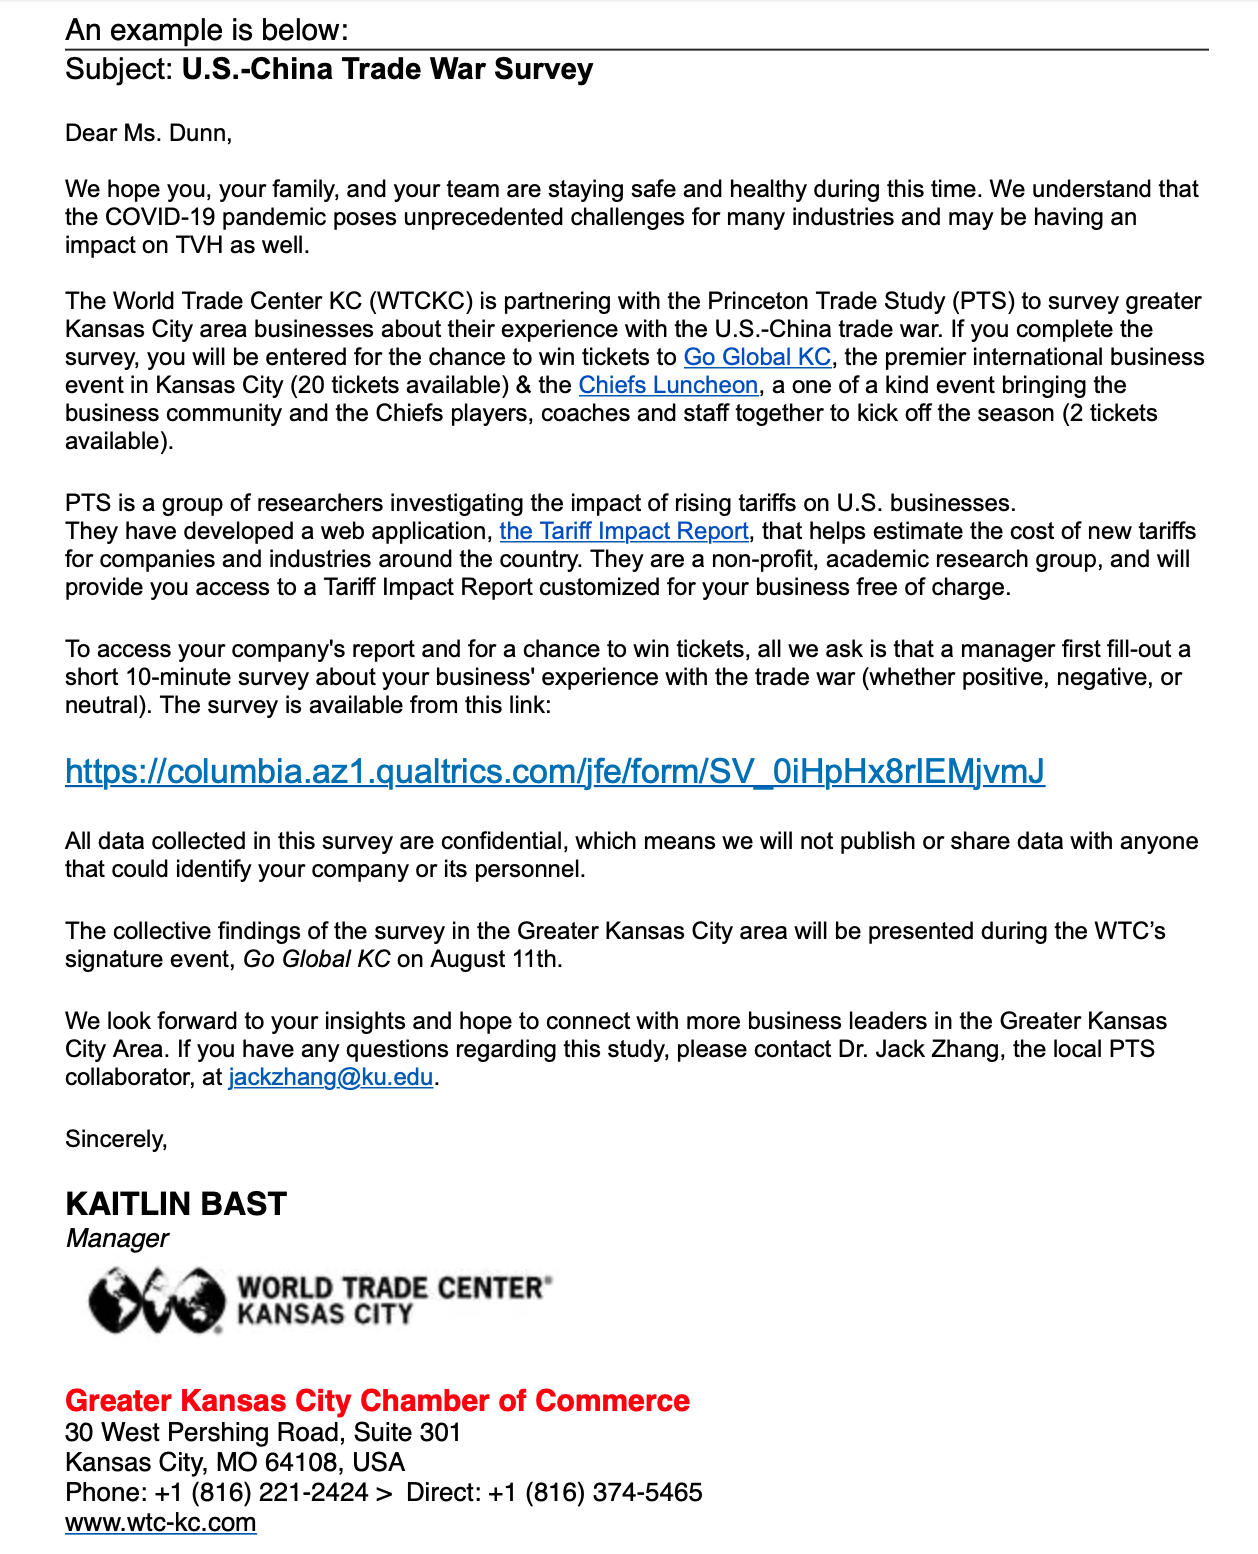
\includegraphics[scale=.5]{KC chamber email.png}
    \caption{Sample Personalized Email from KC Chamber}
    \label{fig:kcchamber}
\end{figure}

\subsection{Outreach via Targeted Facebook Ads}

Targeted ads on Facebook proved to be our most effective sampling strategy. During 2019, we also experimented with contacting managers through Twitter or LinkedIn but found Facebook to be the most cost-effective. We paid to target ads at managers in the United States. We ran two rounds of targets ads on Facebook in June 2019 and July 2020. 

We over-incentivized the first round of sampling by offering a \$5 gift Amazon card. A large number of participants lied about being a manager in order to obtain the reward. We describe below the methods we used to cull the 1747 responses obtained from this wave down to 603 valid responses. We also ran a second round of ads without any incentives one year later, after the Phase One Trade Deal was signed and the onset of the COVID-19 pandemic exacerbated supply chain issues. This wave yielded 335 valid responses. It is hard to calculate a comparable completion rate for the Facebook sample. But we calculate it to be 938 responses from 100,000? impressions. This is a comparably low completion rate as the validated email outreach but much more cost effective.    

\subsection{Validation of Facebook Sample}

Research assistants at the University of Kansas and Wesleyan University helped devise a system for detecting suspicious responses from the Facebook sample based on total response time, IP addresses, and verifying the business name or manager email. The criteria for whether or not a response was invalid are as follows (need two hits to be deemed invalid): 

1) \textit{total response time} - flagged responses under 120s as having a high probability of professional survey taker. Some justification for this: the non-facebook sample had a median response time of 375s, the invalid Facebook responses had a median of 188s. Removing these the Facebook sample has a median response time of 261s 

2) \textit{googling the business name or follow up email} - our RAs did a really good and through job, here are some of my favorite notes: 
- Followed up by e-mail and she is a part-time cannabis trimmer 
- Blogger. in her words "I am not a professional nail artist or anything, it's just a hobby.”
- Facebook page is clearly one baking student
- Domain name is porn
- Reposts where to answer surveys for cash 

3) \textit{identifying duplicate or suspicious IP addresses} - many of the multiple IP hits came from Brazil, Mexico, Venezuela, Australia, these are flagged as invalid 

After applying this screening process, we ended up with 603 valid responses. 
Invalid: 576 responses - flagged for two or more reasons 
Maybe: 568 responses - unable to verify information, usually because no email was provided OR not employed at a business (ex. School, church, non-profit) 
Valid: 603 responses - basically anyone who is real and not trying to scam us: includes not manger, includes many one person "businesses"

The median response time for the valid Facebook sample is 261 seconds compared to 375 seconds for the non-Facebook sample (Email, Phone, KC Chamber). The median size of the valid Facebook sample is 8 employees, the mean is 3160. The median size of the non-facebook sample is 7 employees, and the mean is 7539. The median tariff impact (hurt\_trade) of the valid Facebook sample is 5 (neither), the mean is 4.45 (somewhat harmed). The median tariff impact of the non-facebook sample is 4 (somewhat harmed), the mean is 3.85. This is very promising and suggests that the two are comparable for external validity purposes.  

%Non-facebook sample: 136 
%Orbis Email blast: 2 
%Orbis Phone sample: 68 
%KC Chamber Email + Social Media: 66
%Median response time: 375 seconds 

%Facebook sample: ~605-653
%Median response time: 261 seconds (drop invalids, median of 188s) 


\section{Calculating Industry-Specific Costs of Tariffs}

Our goal was to estimate the costs of the trade war for a highly specific industry.

We began by creating an index of all the unique industries we wanted to generate estimates for. In the original version of our project, our sample was to be a random sample of all firms in Orbis. Even though we ended up pivoting to a primarily Facebook sample, the random sample from Orbis provided the original index of industries we estimated tariff costs for. Our Orbis sample was so large that we caught most industries using this approach. Only about 10\% of our Facebook sample provided an industry for which we were missing estimates.

Next, we wished to identify the input industries to each industry represented in the Orbis data. To do this, we turned to the Bureau of Economic Analysis Input-Output Use Table from 2012.\footnote{Available at \url{https://www.bea.gov/industry/input-output-accounts-data}.} (As of 2019, 2012 was the most recently available year for a widespread group of industries.) The Use tables provide, for every industry, the quantity that industry uses from other industries (see Figure \ref{fig:bea}).

\begin{figure}
    \centering
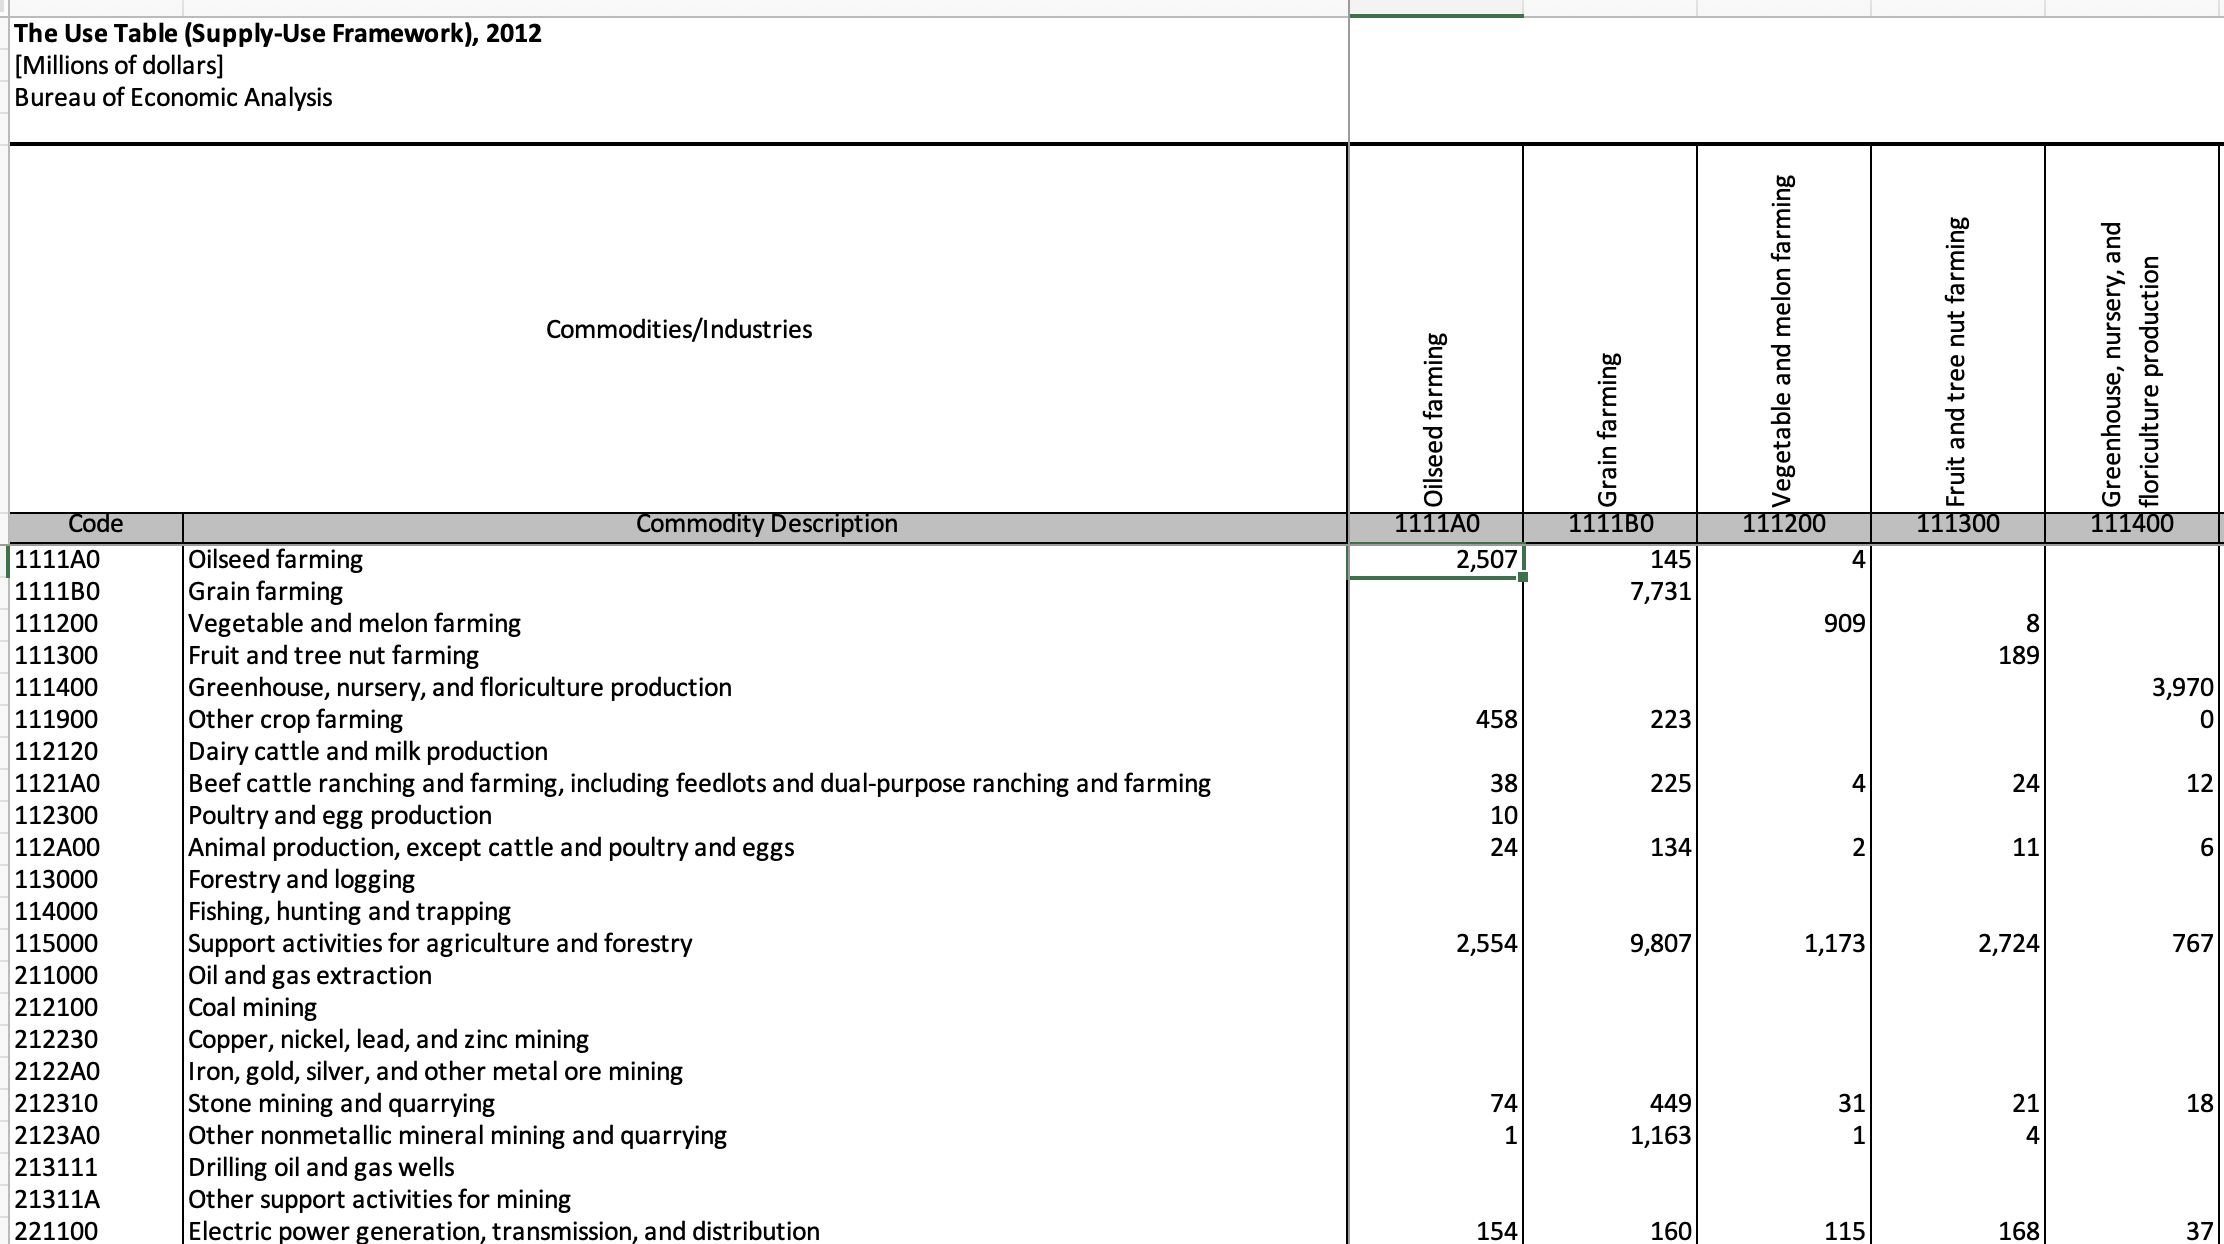
\includegraphics[scale=.4]{bea.png}
    \caption{BEA Use Table}
    \label{fig:bea}
\end{figure}

We merged the NAICS codes from Orbis and the NAICS codes from the BEA at the 3-digit level. This resulted in matches for 94\% of the industries from the Orbis data. When we merged at the 6-digit level, we found matches for only 17\% of the industries from the Orbis data. Since we merged at the 3-digit level, we aggregated the quantities from input industries as reported in the BEA for each 3-digit industry.

Once we knew which input industries each industry relied on, we wanted to know which commodities were associated with each input industry. We did this using a concordance from \cite{pierce2009concording}.\footnote{Available at \url{http://faculty.som.yale.edu/peterschott/sub_international.htm}.} The concordance identifies for each industry (6-digit NAICS) the various commodities associated with that industry (HTS codes) (see Figure \ref{fig:concordance}. We aggregate industries to the 3-digit level to merge with our previous data.

\begin{figure}
    \centering
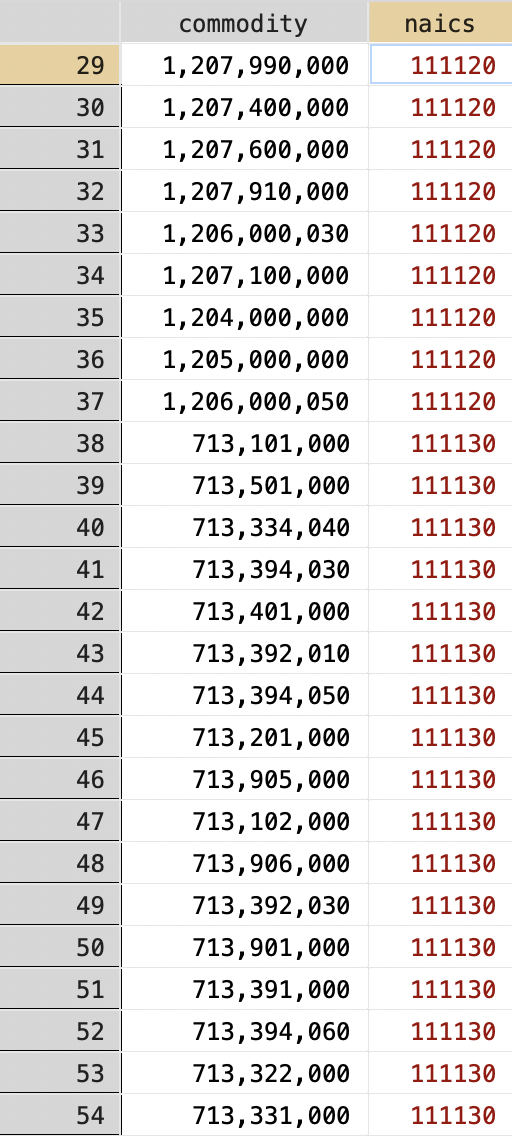
\includegraphics[scale=.4]{concordance.png}
    \caption{Concordance from Pierce and Schott (2009)}
    \label{fig:concordance}
\end{figure}

Last, we wanted to know whether each commodity associated with an input industry was subject to a tariff. We used data made available by Chad Bown at the Peterson Institute for International Economics.\footnote{Available at \url{https://piie.com/system/files/documents/bown2019-02-14.zip}.} An example appears in Figure \ref{fig:bown}. The data indicate which of the various tariff lists each commodity appears on (1) or does not appear on (0).

\begin{figure}
    \centering
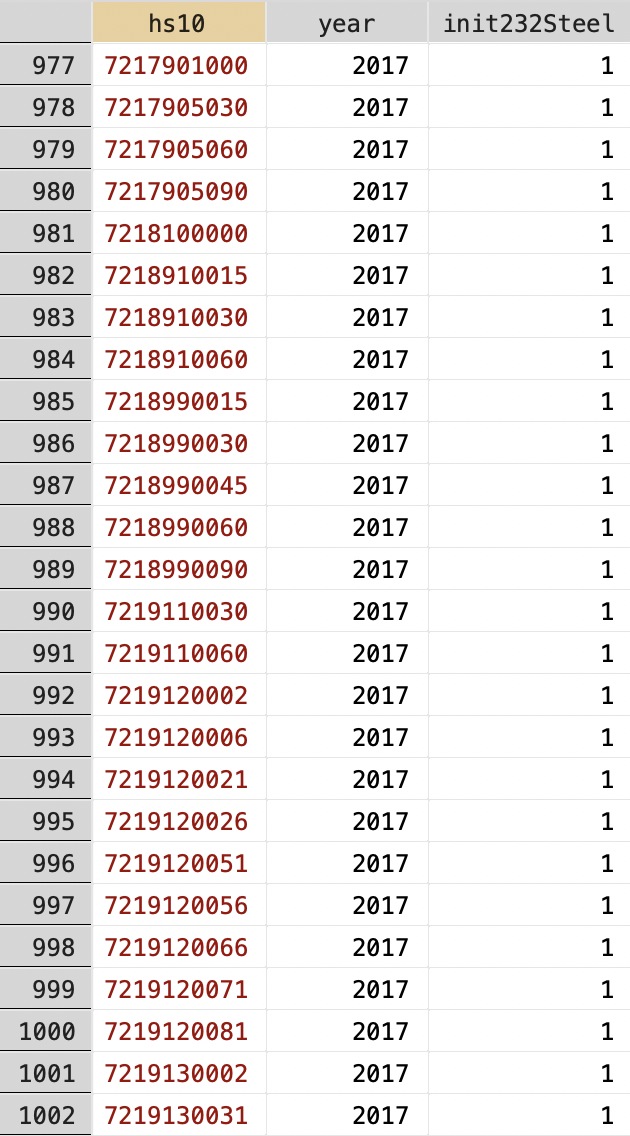
\includegraphics[scale=.4]{bown.png}
    \caption{Tariff Lists from Bown and Zhang}
    \label{fig:bown}
\end{figure}

These data allowed us to estimate, for each input industry, how many commodities it was associated with, how many of those commodities appeared on tariff lists, and the average tariff rate of the lists its commodities appear on. As we explain in the main paper, we summarize this to respondents as the number of tariffed products, the proportion of tariffed products, and the average tariff rate.

We did not want to overwhelm respondents with information, and we did want to provide them with information that would encourage them to act to oppose the trade war. For these reasons, we chose to share with respondents the estimates for the input industries that had the highest proportion of tariffed products (Figure \ref{fig:treatment_pic}). We ordered them first according the highest proportion of tariffed products and second according to which input industries were of greatest value to the industry in question.

\begin{figure}
    \centering
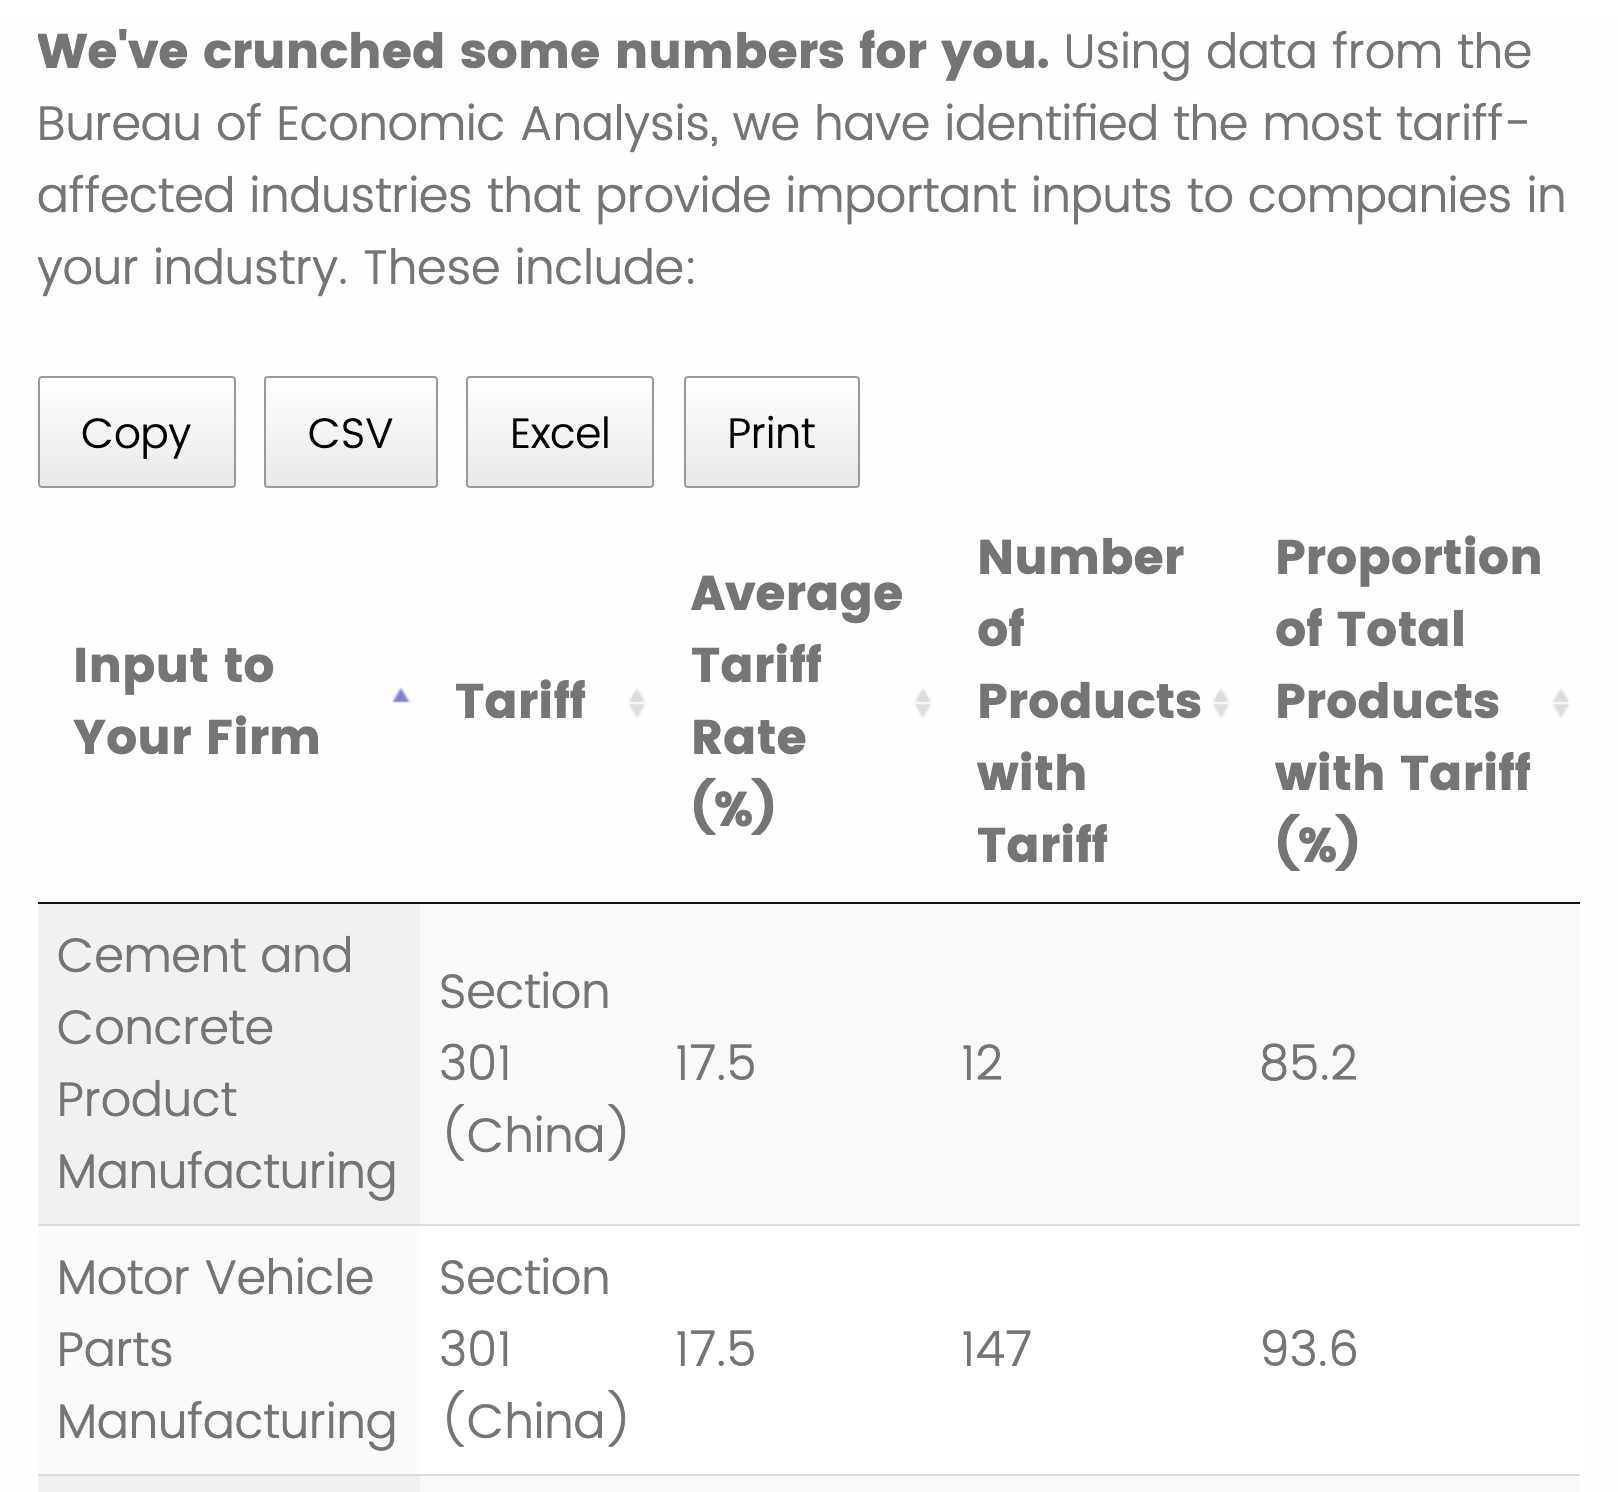
\includegraphics[scale=.4]{treatment_pic.png}
    \caption{Example of Static Treatment}
    \label{fig:treatment_pic}
\end{figure}

\section{ATEs for Support Trade War Outcomes}

In this section we include supplementary results for our support for the trade war outcome, along with a different operationalization of the outcome that looks at the count of outcomes for support or oppose was selected versus whether any one outcome was selected.

\input{tables/all_supp}
\input{tables/collapse_supp}
\input{tables/count_mods}

\section{Model Coefficients for Curvilinear Interactions}

In this section we show the underlying model results for Figures 4 and 5 in the main text.

\input{tables/out_mod_curv}

\section{Model Results for Number of Tariffs Shown}

In this section we report the full model results for our models estimating the effect of the number of tariffs shown to respondents.

\input{tables/mod_treat_opp}
\input{tables/mod_treat_supp}

\section{Additional Treatment Heterogeneity}

In this section we plot the sample average marginal effects of the treatment conditional on varying values of the harm imposed by the trade war in Figure \ref{qopp} and conditional varying values of knowledge of the trade war in Figure \ref{qsupp}.

As noted in Hypothesis 2, or prior expectation was that we would observe a concave-downward shape for the plot. Instead, we see a convex plot with higher values at either extreme for the treatment effect. For those who said that they believed the trade war had affected their firm moderately, it tended to reduce their tendency to oppose the trade war. We note that this finding does not invalidate the simple model we outlined in earlier; rather, our supposition about how prior beliefs would interact with the treatment proved incorrect. Prior beliefs about the effect of the trade war on the firm are very important; those in the middle of the scale experienced a -10 pp decline willingness to oppose the trade war, while those at either end experienced a +10 pp increase in willingness to oppose the trade war upon receiving the treatment. What we did not have accurate information on was which of our respondents was likely to hold overly inflated views of the potential cost of the trade war.

We repeat the same analysis in Figure \ref{qsupp}, although here we do not observe the characteristic U-shape indicative of a quadratic relationship. The treatment's effect does not vary as much depending on respondents' prior beliefs. To the extent that it does, those who believed they were harmed were more likely to oppose the trade war after viewing the treatment, and those who believed they were helped were less likely to oppose the trade war after viewing the treatment. However, as the relationship is very imprecise, we hesitate to assign any concrete interpretation. As mentioned earlier, we did not expect the treatment to have as large an effect on either reducing or increase support for the trade war compared to encouraging opposition.

\begin{figure}
    \centering
    \includegraphics[width=0.7\linewidth]{figures/quad_oppose.png}
    \caption{Conditional Marginal Effect of Treatment on Opposing Trade War by Prior Hurt From Trade War}
    \label{qopp}
\end{figure}

\begin{figure}
    \centering
    \includegraphics[width=0.7\linewidth]{figures/quad_support.png}
    \caption{Conditional Marginal Effect of Treatment on Supporting Trade War by Prior Hurt From Trade War}
    \label{qsupp}
\end{figure}


\section{Analyzing Knowledge and Prior Beliefs}


Tables \ref{learnmod} and \ref{tabmod} show the factors that seems to be associated with a respondent's self-assessed knowledge of the trade war and their prior beliefs about the effect the trade war has had on their company. Table \ref{learnmod} shows that there are several strong predictors of self-assessed knowledge and smaller yet still precise predictors of a respondent's prior beliefs about the trade war's effects (larger values indicate prior belief of help). For knowledge, respondents who were managers, worked at more conservative companies, were members of business associations and had taken political action related to the trade war were more likely to report knowing more about the trade war. As for a respondent's prior beliefs, being in management is not associated with varying beliefs about the trade war, but companies that belonged to associations and had taken action on the trade war were more likely to believe it was beneficial to them. This pattern corresponds to thinking that companies face collective action dilemmas with trade wars, i.e., those companies that are most likely to take action are those that receive concentrated benefits rather than those that pay diffuse costs.

It is interesting to note differing relationships for political ideology between knowledge and prior beliefs (the baseline category is conservative). Respondents who work at conservative companies, compared to those who work at liberal companies, tend to report higher levels of knowledge about the trade war. However, it is respondents who work for moderate firms who believe the trade war has harmed them the most, when compared to both liberal and conservative firms.

\input{tables/learn_pred_tab}

Since we know each respondent's industry, we are also able to explore whether their prior beliefs about the effects of the trade war align with our own assessment (the number of tariffed input products in their industry). Table \ref{tabmod} shows that there does appear to be a quadratic relationship between a respondent's belief in the efficacy of the trade war and the number of products as inputs to their industry with tariffs. The quadratic relationship shows that it varies from the top end to the bottom end of the scale. At a belief of 0 in the benefits of the trade war (i.e. the trade war hurt the firm), the association is strongly positive at $+0.511$, $(+0.109, +0.914)$. For those with a belief of 10 in the benefits of the trade war, the association is strongly negative at  $-0.422$, $(-0.754, -0.09)$. This implies that respondents who worked at firms that had large numbers of tariffs on input products were also more likely to believe, prior to receiving the treatment, that the trade war had already harmed their firm. This analysis provides some evidence that respondents' information about the trade war was at least partly accurate as defined by our data on input tariffs.

We did not find a similar relationship, however, between self-assessed knowledge of the trade war and the number of input products.

\input{tables/tariff_mod}

\section{Sample Inclusion Robustness}

In this section we report headline (ATE) results for our data in which we exclude respondents who listed ``Other" as a NAICS code and respondents who did not meet even more strict validation criteria, such as not being able to ascertain which company the individual worked at. These latter individuals likely are businesspeople; it is simply that we could not verify their position at the their company where they said they worked using secondary sources (i.e. corporate web pages). Tables \ref{oppother} and \ref{suppother} show the opposition and support trade war ATEs with respondents who listed NAICS code as ``Other" removed from the sample. Tables \ref{oppstrict} and \ref{suppstrict} show the opposition and support trade war ATEs by removing respondents who did not meet the strictest set of validation procedures.

In all cases, while significance varies, generally agree with those reported in the main text. When ATEs are significant for opposition to the trade war, the effects are negative. Given the smaller sample sizes, effects tend to be estimated less precisely.

\input{tables/all_opp_other}
\input{tables/all_supp_other}
\input{tables/all_opp_strict}
\input{tables/all_supp_strict}




%\appendix

\end{document}
